%
% Szablon, v. 2.9
% p.wlaz@pollub.pl
%

% PROSZĘ NIE USUWAĆ
% KOMENTARZY Z~PREAMBUŁY
% JEŻELI KTOŚ WAM WMAWIA, ŻE
% TO PRZYSPIESZY COKOLWIEK
% -- MYLI SIĘ!


\documentclass[12pt]{mwbk}


%%%%%%% marinesy, rozmiary, to warto dopasować do drukarki
\usepackage[a4paper,twoside,top=2.6cm,bottom=2.6cm,inner=3cm,outer=2.6cm]{geometry}

%%%%%%%% polszczyzna
\usepackage[T1]{polski}


%%%%%%%%% sposób kodowania literek w edytorze
\usepackage[utf8]{inputenc}

\usepackage[font=small,labelfont=bf,justification=centering]{caption}


%%%% gdyby ktoś chciał powyklejać z~pedeefa
%%%% teksty za pomocą AcroReadera, to 
%%%% poniższe dwie linijki pomogą w~tym
%%%% Może to być przydatne, gdyby ktoś na podstawie
%%%% elektronicznej wersji chciał przygotować dane do 
%%%% badania antyplagiatowego
%%%% ponieważ prace są w
%%%% tych czasach różnymi
%%%% programami antyplagiatowymi
%%%% proszę absolutni NIE
%%%% USUWAĆ następujących
%%%% dwu linijek
\input glyphtounicode.tex
\pdfgentounicode = 1

%%%%%%%%%%%%%%%%%%%%%%%%%%%%%%%%%%%%%
%%%%% jeśli chcesz by główny tekst oraz wzory matematyczne były
%%%%% składane czcionką typu Times Roman (w~odróżnieniu od standardowej
%%%%% TeXowej, czyli Computer Modern Roman) to linia poniżej
%%%%% ma być 'aktywna', następna nieaktywna, 
%%%%% jeśli zrobisz odwrotnie (pierwsza nieaktywna,
%%%%% druga aktywna) uzyskasz skład czcionką
%%%%% Computer Modern Roman mającą wielu wiernych
%%%%% fanów w~świecie TeXa). Konsekwencją jednak będą zmiany
%%%%% rozmiarów czcionek dla rozdziałó i podrozdziałów - rzecz bez większego
%%%%% znaczenia, wynikająca z pewnych zaszłości historycznych (ComputerModern
%%%%% niegdyś były używane wyłącznie w postaci tzw. bitmap)
%\usepackage{mathptmx} \usepackage{tgtermes}
\usepackage{lmodern}

%%% WSZELKIE ZMIANY W~PREAMBULE RÓB ROZWAŻNIE
%%% NIE JESTEŚ PEWNY/PEWNA ICH EFEKTU TO~SPRAWDŹ 
%%% CZY W~PRGRAMIE ADOBE READER (i~to dokładnie
%%% o~ten program chodzi, nie o~jakikolwiek)
%%% Z~WYNIKOWEGO PLIU PDF DA SIE PRAWIDŁOWO
%%% WYKLEIĆ TEKST Z~POLSKIMI LITERAMI, BEZ KRZAKÓW,
%%%% BEZ DZIWACTW.


%%%%%%%%%%%%%% pozostałe pakiety używane w~pracy, to już zależy od
%%%%%%%%%%%%%% autora, więc może być tego więcej
\usepackage{fancyhdr}
\usepackage{graphicx}
\usepackage{amsmath}
\usepackage{amsthm}
\usepackage{amssymb}
\usepackage{url}
\usepackage{longtable}
\usepackage{array,hhline}
\usepackage{tabu}


%%%%%%%% hyperref po to by przeglądarka pedeef ukazywala na odwołania
%%%%%%%% prawidłowo skonstruowane za pomocą \ref, \cite i.t.d. jako
%%%%%%%% hiperłącza
\usepackage{hyperref}



%%%%% dla fanów ``profesjonalnych'' tabel w~stylu zachodnich książek

\usepackage{booktabs} \heavyrulewidth=1.5bp \lightrulewidth=0.5bp


%%%%%%%%%%% poniżej uniwersalny sposób na ucywilizowanie znaków 
%%%%%%%%%%% niewiększości, niezależny od pakietu {polski}, ale za to 
%%%%%%%%%%% zależny od {amssymb}, ma tą zaletę, że działa np. z Timesem
%%%%%%%%%%% w matematyce
\let\leq\leqslant\let\le\leq\let\geq\geqslant\let\ge\geq


%%%%%%% jeżeli będziesz chciał włączać do swojej pracy fragmenty programów, 
%% to ponizsza linijka przyda się, jeśli nie - usuń ją

\usepackage{fancyvrb}


%%%%%%%%%%%%%%%%% struktury do tworzenia twierdzeń i~tym podobnych

\theoremstyle{plain}
\newtheorem{twier}{Twierdzenie}[chapter] % pierwsze to nazwa środowiska,
                                      %drugie to wyświetlana nazwa
				% to trzecie w~nawiasie kwadratowym
				% wskazuje numer dolepiony z~lewej do
				% numeru twierdzenia (tu numer
				% 'chapter', 
\newtheorem{lemat}{Lemat}[chapter]

\theoremstyle{definition}
\newtheorem{defi}{Definicja}[chapter]

\theoremstyle{remark}
\newtheorem{uwaga}{Uwaga}[chapter]
\newtheorem{wniosek}{Wniosek}[chapter]

%%%%% więcej możliwości w~dokumentacji amsthm



%%%%%%%%%%%%%%%%%%%%%%%%%%%%%%%%%%%%%%%%%5
%%%%%%%%%%%%%%%%%%%%%%%%%%%%%%%%%%%%%%%%%%
%%%%%%%%% wcięcie akapitowe %%%%%%%%%%%%%%
%%%%%%%%%%%%%%%%%%%%%%%%%%%%%%%%%%%%%%%%%%
%%%%%% ustawić w~zaleceń i~gustu %%%%%%%%%
%%%%%%%%%%%%%%%%%%%%%%%%%%%%%%%%%%%%%%%%%%
%%%%%%%% zalecenie na stronie wydziałowej
%%%%%%%% było 1.25cm i wyglądało jakoś 
%%%%%%%% śmiesznie duże, więc spłoszony nieco
%%%%%%%% wpisałem 1cm, ale uważny czytelnik już
%%%%%%%% zapewne się domyśli, że podmiana napisu 
%%%%%%%% =1cm na =1.25cm sprawi, że wcięcia na początku
%%%%%%%% akapitu ustawią się na (nieco przydużą)
%%%%%%%% wartość 1.25cm 

\parindent=1cm



%%%%%%%%%%%%%%%%%%%%%%%%%%%%%%%%
%%%%% tu pewne poluzowanie rozmieszczenia elementów tabelek
%%%%% możecie sobie poeksperymentować, by dopasować do swych
%%%%% gustów, a przede wszystkim gustów promotorów (promotorek)
  \tabcolsep=4mm          
  %\renewcommand\arraystretch{1.3}
%%%%%%%%%%%%%%%%%%%%%%%%%%%%%%%%%%



%%%%%%%%% teraz żywa pagina (aka 'running headline') i~numerowanie stron
%%%%%%%%%%%%%%%%%%%%%%%%%%%%%%%%%%%%%%%%%%%%%%%%%%%%%%%%%%%%%%%%%%%%%%%%
%%%%%na górze mają być śródtytuły, na dole (po stronie zewneętrznej)
%%%%%numery stron. Poszedłem kapkę dalej i~na stronach ropoczynających
%%%%%rozdział nie ma paginy (górki).
%%%%% Oczywiście jeśli ostatnia strona
%%%%% jest pusta (uzupełnia jeno parzystość) to tam żadnej stopki ani 
%%%%% górki byc mnie może - ma być pusta.
%%%%%%%%%%%%%%%%%%%%%%%%%%%%
\pagestyle{fancy}
\fancyhead{}% oczyszczenie
\fancyhead[RO]{\rightmark} %% na nieparzystych 'podległe' śródtytuły
\fancyhead[LE]{\leftmark} %% na parzystych 'ważniejsze'
\fancyfoot{}% oczyszczenie
\fancyfoot[RO,LE]{\arabic{page}}  %% numer na dole (po prawej na
%% nieparzystych, po lewej na parzystych)
\renewcommand\headrulewidth{0.4pt} %%% cienka hrulka oddzielająca paginę
                                    %%% od kolumny tekstu
\fancypagestyle{closing}{%%%%%% to styl dla stron zamykających rozdział
\fancyhead{}% oczyszczenie
\fancyhead[RO]{\rightmark} %% na nieparzystych 'podległe'
\fancyhead[LE]{\leftmark} %% na parzystych 'ważniejsze'
\fancyfoot{}% oczyszczenie
\fancyfoot[RO,LE]{\arabic{page}}  %% numer na dole (po prawej na
                                  %% powyższą linijkę usuń jeśli nie
				  %% chcesz numerów na niepełnych
				  %% kolumnach (zamykających rozdział)
\renewcommand\headrulewidth{0.4pt}
}
\fancypagestyle{opening}{%%% styl stron rozpoczynających rozdział
\fancyhead{}% oczyszczenie
\fancyfoot{}% oczyszczenie
\fancyfoot[RO,LE]{\arabic{page}}  %% numer na dole (po prawej na
\renewcommand\headrulewidth{0pt}
}
\fancypagestyle{plain}{%%%% styl zwykły, niektóre konstrukcje
                       %%%% (typu \titlepage, którego ja tu nie używam
                       %%%% ale może są jakieś inne o których nawet nie chce 
                       %%% mi się myśleć, więc dla spokoju robię to po swojemu
\fancyhead{}% oczyszczenie
\fancyfoot{}% oczyszczenie
\fancyfoot[RO,LE]{\arabic{page}}  %% numer na dole (po prawej na
\renewcommand\headrulewidth{0pt}
}

%%%%%%%%%%%%%%%%%%%%%%%%%%%%%%%%%5
%%%%%%%%%%%%%%%%%%%%%%%%%%%%%%%%%%
%%% lekka modyfikcja 'markow' do paginy
%%% uznalem, ze jesli ktos nie da \section (np we wstepnie czy
%%% podsumowaniu to niech na obu sronach w~paginie pojawia sie tytuł
%%% chaptera, bo standardowo, to na nieparzystej stronie w takiej sytuacji
%%% nad górną linią ziałaby pustka, co mogłoby wprowadzać konsternację
\makeatletter
    \def\chaptermark#1{%
      \markboth{%
        \ifHeadingNumbered
     \if@mainmatter
     \@chapapp\
            \thechapter.\enspace
          \fi
        \fi
        #1}{%
        \ifHeadingNumbered
     \if@mainmatter
     \@chapapp\
            \thechapter.\enspace
          \fi
        \fi
        #1%
	}}%
    \def\sectionmark#1{%
      \markright{%
        \ifHeadingNumbered \thesection.\enspace \fi
        #1}}
%%%%%%%%%%%%%%%%%%%%%%%%%%%%%%%%%%%%%%%%%%%%%%%
%%%%%%%%%%%%%%%%%%%%%%%%%%%%%%%%%%%%%%%%%%%%%%%%
%%%%%%%%%%%% wielkości czcionek dla chapter i~section
%%%%%%%%%%%% 16 dla rozdziału, 14 dla podrozdziału - te domyślne
%%%%%%%%%%%% w klasie mwbk były całkiem ładne, ale żeby nie było
%%%%%%%%%%%% że nie potrafię ustawić
%%%%%%%%%%%%%%%%%%%%%%%%%%%%%%%%%%%%%%%%%%%%%%%%%%%
\SetSectionFormatting[breakbefore,wholewidth]{chapter}
        {0\p@}
        {\FormatRigidChapterHeading{6.4\baselineskip}{12\p@}%
	{\large\@chapapp\space}{\fontsize{16}{19}\selectfont}}
        {1.6\baselineskip}
\SetSectionFormatting{section}
        {24\p@\@plus5\p@\@minus2\p@}
	{\FormatHangHeading{\fontsize{14}{16}\selectfont}}
        {10\p@\@plus3\p@}
\makeatother	



%%%%%%%%%%%%%%%%%%%%%%%%%%%%%%%%%%%%%%%%%%%%%%
%%%%%%%%%%%%%%%%%%%%%%%%%%%%%%%%%%%%%%%%%%%%%%
%%%%%%%%%%%%%% jakies inne pomocnicze definicje, ja na przykład lubię
% \R
%%%%%%%%%%%%%%%%%%%%%%%5
%%%%%%%%%%%%%%%%%%%%%%%
%%%% tak naprawdę są t potrzebne tylko po to
%%%% by zadziałały przykłady poniżej w tekście
%%%% które w sposób dość losowy zostały 
%%%% pobrane z jakichś moich starych plików
%%%%%%%%%%%%%%%%%%%%%%%%%%%%%%%%%%
%%%%%%%%%%%%%%%%%%%%%%%%%%%%%%%%%%%
%%%% w realnej pracy te poniższe śmieci możecie oczywiście
%%%% usunąć
%%%%%%%%%%%%%%%%%%%%%%%%%%%%
\newcommand\R{\mathbb{R}}
\newcommand{\ff}{\mathbf{f}}
\newcommand{\hh}{\mathbf{h}}
\newcommand{\xx}{\mathbf{x}}
\newcommand{\yy}{\mathbf{y}}
\newcommand{\zz}{\mathbf{z}}
\newcommand{\gggg}{\mathbf{g}}
\newcommand{\skalar}[2]{\pmb{\langle}#1,#2\pmb{\rangle}}
%%%%%%%%%%%% koniec tych dodatkowych definicji

%%%%%% trocę więcej ``luzu'' przy rozmieszczaniu {fgur} i~{table}

 \renewcommand{\topfraction}{0.9}	% max fraction of floats at top
    \renewcommand{\bottomfraction}{0.8}	% max fraction of floats at bottom
    %   Parameters for TEXT pages (not float pages):
    \setcounter{topnumber}{2}
    \setcounter{bottomnumber}{2}
    \setcounter{totalnumber}{4}     % 2 may work better
    \setcounter{dbltopnumber}{2}    % for 2-column pages
    \renewcommand{\dbltopfraction}{0.9}	% fit big float above 2-col. text
    \renewcommand{\textfraction}{0.07}	% allow minimal text w. figs
    %   Parameters for FLOAT pages (not text pages):
    \renewcommand{\floatpagefraction}{0.7}	% require fuller float pages
    % N.B.: floatpagefraction MUST be less than topfraction !!
    \renewcommand{\dblfloatpagefraction}{0.7}	% require fuller float pages
    % remember to use [htp] or [htpb] for placement

    
%%% DWA proste polecenia służące do ujednolicenia podawania źródeł przy rysunkach i~tabelkach    
    
    \newcommand\zrodlo[1]{\par\vspace{-3mm}{\small\textit{Źródło: }#1 }}
    \newcommand\zrodlotab[1]{{\par\vspace{2mm}\small\textit{Źródło: }#1 }}

\raggedbottom   %%% to znaczy, że nie będzie siłowego wyrównywania typowych
                %%     stron do jednakowej wysokości

\linespread{1.3}

\begin{document}

%%%%%%%%%%%%%%%%%%%%%%%%%%%%%%%%%%%%%%%%%
%%%%%%%%%%%%%%%%%%%%%%%%%%%%%%%%%%%%%%%%%
%%%%%%%% STRONA TYTUŁOWA %%%%%%%%%%%%%%%%

\thispagestyle{empty}  % tu wszak nie chcemy żadnej numeracji stron


%%%%%%%%%%%%%%%%%%%%%%%%%%%%%%%%%%%%%%%%%%%%%%%%%%%%%%%%%%%%%%%
%%%%%tytuły definiuje jako makrodefinicje, gdyż zamierzam je%%%
%%%%%powtórzyć na stronie ze streszczeniami, to nic nie boli%%%
%%%%%a gwarantuje, że będą one takie same, i~tak ma być.%%%%%%%
%%%%%%%%%%%%%%%%%%%%%%%%%%%%%%%%%%%%%%%%%%%%%%%%%%%%%%%%%%%%%%%
\newcommand\tytul{Zastosowanie modeli mieszanych w analizie rozwoju pandemii choroby COVID-19 na świecie}

\newcommand\tytulangielski{The Use of Mixed-Effects Models in the Analysis of the COVID-19 Pandemic in the World}


\begin{center}


{\large \bf POLITECHNIKA LUBELSKA}

{\bf WYDZIAŁ PODSTAW TECHNIKI}

\emph{Kierunek:} MATEMATYKA

%%% BEZ SPEC.!!! \emph{Specjalność:} Matematyka w~finansach i~ubezpieczeniach

\vfill %%%% \vfill to taki rozpychacz w pionie, pcha ile mu pozwolą
     


\includegraphics[width=3.5cm]{rys/logopl}

\vfill

\textbf{Praca inżynierska}

\vfill
\vfill
\vfill

\large
\tytul

\vfill

\emph{\tytulangielski}


\vfill
\vfill
\vfill
\vfill
\vfill

\begin{tabular}[t]{l}
\emph{Praca wykonana pod kierunkiem:}
\\
dra Dariusza Majerka
\end{tabular}
\hfill
\begin{tabular}[t]{l}
	\emph{Autor:}
\\
Alicja Hołowiecka\\
nr albumu: 89892 
\end{tabular}

\vfill
\vfill
\vfill

\textbf{Lublin 2020}

\end{center}


%%%%% koniec tytułów


%%%%%%%%%%%%%%%%%%%%%%%5
%%%%%%%%%%%%%%%%%%%%%%
%%% teraz spis treści
%%%%%%%%%%%%%%%%%%%%%
%%% pamiętaj! po jakiejkolwiek zmianie w tekście
%%% która wpływa na zmianę spisu treści, spis będzie dobry co najmniej
%%% po dwóch przebiegach latexa - to samo dotyczy odwołań do wzorów i literatury
%%% ogólnie to przed wydrukiem warto przelatexować o jedne raz więcej niż
%%% to się wydaje konieczne, no chyba że korzystamy z funkcji typu BUILD
%%% w zintegrowanym systemie wspomagającym TeX, BUILD powinien takie sprawy 
%%% wziąć pod uwagę

\tableofcontents


\chapter*{Wstęp}




Pandemia choroby COVID-19 jest wydarzeniem, które wstrząsnęło całym światem w roku 2019. Właściwie nikt chyba nie może powiedzieć, że nie poczuł się dotknięty przez sytuację związaną z rozprzestrzenianiem się wirusa. Pierwsze przypadki pojawiły się pod koniec 2019 roku we wschodnich Chinach, w mieście Wuhan. Na początku 2020 roku chorowali już obywatele większości państw na świecie. Na moment pisania tej pracy, sytuacja nadal nie jest opanowana i nie wiadomo, jak się rozwinie.

Biorąc to pod uwagę, tym ważniejszy wydaje się temat poruszany w tej pracy. Wiele jednostek naukowych podejmuje próby znalezienia odpowiedniego modelu, aby przewidzieć rozwój pandemii. Przedstawione w tej pracy modele mieszane co prawda nie pozwalają na dokładną predykcję, ale są dobrym narzędziem, aby odkryć, które czynniki mają wpływ na rozwój pandemii w przeciętnym kraju.











\chapter{Teoretyczne podstawy badań własnych}
W tej części pracy przedstawimy metody matematyczne, które zostaną użyte w części praktycznej tej pracy. Zgodnie z tematem, będą to głównie modele mieszane.
\section{Modele liniowe}
Na początek przypomnimy podstawowe wiadomości o modelach liniowych.

Model regresji prostej ma postać 
$$y=x \beta_1+\beta_0 + \varepsilon$$

gdzie oszacowania parametrów $\beta_1$, $\beta_0$ obliczamy następująco:

$$\hat{\beta_1}=\frac{Cov(x,y)}{Var(x)},$$
$$\hat{\beta_0}=\overline{y}-\overline{x}\hat{\beta_1}.$$

Model interpretujemy w ten sposób, że jeżeli zmienna $x$ wzrośnie o 1, to zmienna $y$ zmieni się o $\beta_1$.

Zmienną $y$ nazywamy zmienną zależną, a $x$ - niezależną.

Jeżeli w modelu występuje więcej niż jedna zmienna niezależna, to mówimy o regresji wielorakiej (lub wielokrotnej). Wówczas model ma postać:

$$y=\beta_0+\beta_1 x_1+\beta_2 x_2 + \ldots + \beta_k x_k + \varepsilon,$$
lub w zapisie macierzowym
$$\yy=\mathbf{X}\beta+\varepsilon$$
\subsection{Metody estymacji parametrów modelu liniowego}
\begin{enumerate}
	\item Metoda najmniejszych kwadratów, OLS (ang. \emph{Ordinary Least Squares}) - w metodzie tej minimalizujemy błąd kwadratowy, czyli sumę kwadratów reszt, którą oznaczamy RSS (ang. \emph{Residual Sum of Squares}).
	
	$$RSS= \sum_{i=1}^{n}(y_i-\hat{y_i})^2$$
	
	Twierdzenie Gaussa-Markowa: taki estymator jest BLUE (Best Linear Unbiased Estimator), przy odpowiednich założeniach.
	
	\item Metoda największej wiarogodności, ML (ang.\texttt{Maximum Likelihood}) polega na maksymalizacji wartości funkcji prawdopodobieństwa ze względu na $\beta$ (w praktyce maksymalizujemy zwykle logarytm z tej funkcji)
	
	$$\hat{\sigma}^{2}_{ML}=RSS/n$$
	
	Estymując $\sigma^2$, maksymalizujemy funkcję wiarogodności zarówno ze względu na $\beta$, jak i $\sigma^2$.
	
	Estymatory uzyskane tą metodą są asymptotycznie nieobciążone.
	
	\item Resztowa metoda największej wiarogodności, REML (ang. \texttt{Residual/Restricted Maximum Likelihood Method}) - z estymacji parametru $\sigma^2$ usuwamy wpływ parametrów zakłócających $\beta$.
	
	$$\hat{\sigma}^2_{REML}=RSS/(n-p)$$
	
	Estymatory uzyskane tą metodą są nieobciążone \cite{biecek}.
\end{enumerate}

\subsection{Badanie istotności parametrów}

Aby zbadać istotność współczynników modelu liniowego, weryfikujemy hipotezę postaci

$$H_0: \beta_i = 0$$

przeciw hipotezie alternatywnej $$H_1: \beta_i \neq 0.																																																																																																																																																																																																																																																																																																																																																																																																																																																																																																																													$$

Do zweryfikowania tej hipotezy wykorzystujemy test Walda.
Statystyka testowa ma postać $$T=\hat{\beta_i}/se(\hat{\beta_i})$$
i jest nazywana statystyką t (ang. \texttt{t-value}).

Przy założeniu prawdziwości $H_0$ statystyka ta ma rozkład t-Studenta o $n-k-1$ stopniach swobody ($n$ - liczba obserwacji, $k$ - liczba parametrów w modelu).

Można także użyć testu F (testu globalnego), aby zweryfikować hipotezę

$$H_0: \beta_1=\beta_2=\ldots=\beta_k=0$$

przeciwko hipotezie alternatywnej
$$H_1: \exists{j} \beta_j \neq 0 $$

\section{Modele mieszane} 
W powyżej opisanych modelach liniowych z efektami stałymi zakładamy niezależność kolejnych pomiarów, dlatego nie są to odpowiednie modele, kiedy mamy np. kilka pomiarów dla pojedynczego elementu. W takim przypadku możemy użyć modeli liniowych z efektami mieszanymi (stałymi i losowymi), które krótko nazywamy modelami mieszanymi.

Modeli mieszanych używamy w przypadu powtarzanych pomiarów bądź w przypadku hierarchicznej lub zagnieżdżonej struktury. Takie dane charakteryzują się korelacją między obserwacjami z tej samej grupy, co nie pozwala na użycie modelu liniowego z efektami stałymi. Dlatego do modelu wprowadza się czynnik losowy. 

Czynnik stały jest pewnym parametrem, którego wartość estymujemy na podstawie próbki, natomiast czynnik losowy jest zmienną losową, dla której próbujemy oszacować parametry jej rozkładu \cite{faraway}.
	
Przykładową sytuacją, gdzie możemy użyć modelu mieszanego, jest badanie działania leku na grupie pacjentów, gdzie dokonujemy kilku pomiarów na danym pacjencie. W tym przypadku nie interesuje nas konkretny pacjent, ale raczej wpływ leku na przeciętnego pacjenta. Dodatkowo, traktujemy pacjentów jako losowo wybranych. Podejście modelu mieszanego będzie polegało na potraktowaniu wpływu pacjenta jako czynnik zakłócający. 

Rozważamy model postaci
$$y=X\beta +Z u + \varepsilon$$
gdzie $X$ - macierz zmiennych będących efektami stałymi, $Z$ - macierz zmiennych będących efektami losowymi, $\beta$ to wektor nieznanych efektów stałych, $\varepsilon \sim \mathcal{N}(0, \sigma^2 I_{n\times n})$ to zakłócenie losowe, a $u \sim \mathcal{N} (0, \sigma^2D)$ to wektor zmiennych losowych odpowiadających efektom losowym \cite{biecek}.

Znając $D$, możemy estymować parametry $\beta$ uogólnioną metodą najmniejszych kwadratóW. Do estymowania nieznanego $D$ możemy użyć np. metodą największej wiarogodności.

\subsection{Metody estymacji}

Do oceny wartości parametrów modelu mieszanego można stosować metody ML (Największej Wiarogodności) oraz REML (Resztowej Największej Wiarogodności), wspomniane w tej pracy przy okazji modeli liniowych. W przypadku modeli mieszanych obydwoma metodami możemy uzyskać estymatory obciążone, ale to obciążenie jest zazwyczaj mniejsze w przypadku estymatorów uzyskanych metodą REML.

Różnica między metodą REML i ML polega na tym, że w metodzie REML najpierw usuwamy wpływ efektów stałych, które w modelach mieszanych są czynnikami zakłócającymi.

\subsection{Badanie istotności parametrów i wybór najlepszego modelu}

W modelach mieszanych konieczne jest zbadanie istotności dla efektów stałych oraz dla efektów losowych.

Dla efektów stałych testujemy hipotezę

$$H_0: \beta_i=0$$

przeciwko hipotezie alternatywnej $$H_1: \beta_i \neq 0,$$

a dla komponentów wariancyjnych weryfikujemy hipotezę

$$H_0: \sigma^2_j=0$$

przy jednostronnej hipotezie alternatywnej 
$$H_1: \sigma^2_j>0.$$



Metody, które mają zastosowanie dla modeli liniowych z efektami stałymi, nie zawsze dają się zastosować w przypadku modeli mieszanych. Wymienimy teraz kilka metod doboru najlepszego modelu i opiszemy, które z nich są najskuteczniejsze \cite{faraway}.

\begin{enumerate}
	\item Iloraz wiarygodności(ang. \texttt{likelihood ratio}) - tworzymy dwa modele, model 0, który nie zawiera elementów, których istotność chcemy zbadać, i model 1, który zawiera te elementy. Pozostałe zmienne muszą być takie same w obu modelach.
	
	Statystyka testowa wygląda następująco:
	$$2(l(\hat{\beta_1}, \hat{\sigma_1}, \hat{D_1}|y)-l(\hat{\beta_0}, \hat{\sigma_0}, \hat{D_0}|y)),$$
	gdzie l - logarytm z funkcji prawdopodobieństwa.
	
	Tego testu nie można używać do modeli wyznaczonych metodą \texttt{REML}.
	
	\item Test F dla efektów stałych - metoda taka sama jak ta używana przy modelach z efektami stałymi. W przypadku modeli mieszanych może sprawiać problemy, ponieważ statystyka testowa niekoniecznie musi mieć rozkład F. Należy także wprowadzać poprawkę na liczbę stopni swobody.
	
	Na ogół ta metoda daje dobre rezultaty dla mniej skomplikowanych modeli, gdy układ jest zbalansowany (wszystkie grupy są równoliczne). Dla modeli bardziej skomplikowanych, lub kiedy brak równoliczności, wartości p oraz statystyki t mogą być błędne.
	
	\item Test permutacyjny - można użyć metod \textit{bootstrapowych}, aby znaleźć dokładniejsze wartości p-value. Należy wygenerować dane z modelu 0 (na podstawie oszacowanych parametrów) i obliczyć statystykę \textit{likelihood ratio}. Tą procedurę powtarzamy wielokrotnie i oceniamy istotność.
	
	\item Kryteria informacyjne - służą do wyboru najlepszego spośród modeli. Najpopularniejszym jest Kryterium Informacyjne Akaikego (ang. \texttt{Akaike Information \\Criterion, AIC}). Jest ono zdefiniowane następującym wzorem:
	
	$$-2(\texttt{max log likelihood})+ 2p,$$
	
	gdzie $p$ to liczba parametrów modelu.
	
	Można stosować to kryterium do modeli, które różnią się jedynie efektami stałymi, gdzie liczba efektów losowych jest identyczna dla wszystkich modeli, które porównujemy. Gdyby modele różniły się liczbą efektów losowych, należałoby rozważyć, w jaki sposób zliczyć liczbę parametrów $p$.
	
	Kryterium Akaikego jest miarą utraconej informacji, więc po obliczeniu go dla roważanych modeli, należy wybrać ten, gdzie otrzymana wartość jest najmniejsza.

\end{enumerate}

Przy obliczeniach dotyczących stosunkowo małych zbiorów danych, można użyć każdej z tych metod, ale w przypadku dużej liczby obserwacji, niektóre obliczenia mogą zająć zbyt wiele czasu. Najmniej skomplikowany obliczeniowo jest test Walda, gdzie dokonujemy tylko jednej estymacji współczynników. Przy użyciu testu ilorazu wiarygodności, należy dokonać dwóch estymacji - dla modelu z i bez testowanego efektu. Stosując testy permutacyjne, musimy dokonać obliczeń setki lub tysiące razy. Dlatego w przypadku najbardziej skomplikowanych problemów zwykle stosuje się test Walda, mimo jego gorszych właściwości statystycznych \cite{biecek}.

\subsection{Interpretacja parametrów modelu mieszanego}
W modelu mieszanym efekty stałe należy interpretować tak jak w przypadku regresji, analizy wariancji lub analizy kowariancji, w zależności od rodzaju zmiennej niezależnej. Trzeba jednak pamiętać, że oszacowane wartości współczynników reprezentują wartość średnią dla całej populacji, a dla poszczególnych obiektów badania będą się różnić o wartość oceny efektu osobniczego.

Dla efektu losowego możemy oszacować jego wariancję. Informuje nas ona o tym, jak bardzo mogą się różnić współczynniki efektów stałych dla poszczególnych obiektów badania
\cite{experimental}.

Można wyróżnić dwa rodzaje efektów losowych: losowy wyraz wolny (rysunek \ref{fig:random_types}, wykres A) oraz losowy wyraz wolny i współczynnik nachylenia (rysunek \ref{fig:random_types}, wykres B). W pierwszym przypadku, prosta regresji dla poszczególnych obiektów badań może być przesunięta w górę lub w dół w stosunku do średniej, a w drugim przypadku może także być nachylona do osi OX pod mniejszym lub większym kątem.

\begin{figure}[htbp]
	\centering
	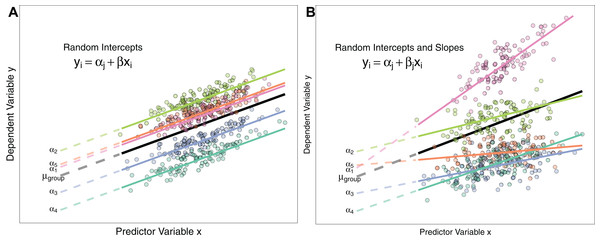
\includegraphics[width=\linewidth]{rys/random_types.jpg}
	\caption{Rodzaje modeli mieszanych}
	\label{fig:random_types}
	\zrodlo{\cite{brief}}
\end{figure}

\subsection{Predykcja z modelu mieszanego}
Proces predykcji jest trudniejszy w przypadku modelu mieszanego niż dla zwykłego modelu liniowego. Musimy zdecydować, czy uwzględnić, czy wykluczyć efekt losowy z predykcji. Efekty losowe mogą mieć różny wkład w predykcję. Mogą być całkowicie pominięte, mogą być uśrednione lub mogą być na pewnym ustalonym poziomie. Uśrednienie efektów losowych powoduje predykcję zależną od wartości efektów losowych, które zostały zaobserwowane do tej pory. Pominięcie efektów losowych powoduje predykcję na poziomie średniej populacyjnej
 \cite{prediction}.
 
 Aby lepiej przybliżyć zagadnienie predykcji z modelu mieszanego, posłużymy się przykładem badania mleczości krów. Dla 10 krów (oznaczonych literami od A do J) zmierzono ilość mleka wyprodukowaną przez każdą z nich w ciągu dnia. Pomiary powtórzono pięciokrotnie \cite{biecek}.
 
 Model ma postać 
 $$y_{milk.amount}=\mu+Z_{cow}u_{cow}+\varepsilon,$$

$$u_{cow} \sim \mathcal{N}(0, \sigma^2_{cow}).$$
 
 Jeżeli chcielibyśmy dokonać predykcji dla nieznanej lub do tej pory niezbadanej przez nas krowy, to wynikiem byłaby ocena średniej dla całej populacji, czyli $\hat{\mu}$.
 
 Aby dokonać predykcji dla konkretnej krowy spośród tych przebadanych, potrzebne nam są oceny efektów osobniczych krów.
 
 Znając macierz $D$ i parametry $\beta$, predykcje efektów losowych $\widetilde{u}$ można wyznaczyć ze wzoru
 
 $$\widetilde{u}=DZ^TV^{-1}(y-X\beta),$$
 gdzie $V$ to macierz $\sigma^2(I+ZDZ^T)$ \cite{biecek}.
 
 Wówczas predykcja będzie sumą $\hat{\mu}$ oraz oceny efektu losowego dla odpowiedniego osobnika.
 
\chapter{Badania własne}
\section{Opis zbioru badawczego}

Zbiór danych pochodzi z witryny internetowej Our World In Data \cite{owid}, gdzie dane zostały zebrane z różnych źródeł, m. in. ze Światowej Organizacji Zdrowia (WHO) oraz Europejskiego Centrum ds. Zapobiegania i Kontroli Chorób (ECDC). W zbiorze znajduje się 210 krajów, dane dotyczące terytoriów międzynarodowych oraz łącznie dla całego świata. Mamy ponad 40 kolumn z różnymi parametrami - w dalszej części pracy opiszemy, które zmienne będą przez nas użyte.

W zbiorze znajdowało się wiele braków danych. Dla każdego kraju zostały usunięte dane sprzed rozpoczęcia się epidemii na jego terytorium (\texttt{total cases=0}), dni są numerowane kolejnymi liczbami całkowitymi.

Ze zbioru danych zostały usunięte wszystkie kraje o populacji poniżej miliona mieszkańców, ponieważ w większości były to nieduże wysepki, dla których dane były wybrakowane. Oprócz tego, kilka innych krajów zostało usuniętych, ponieważ mimo większej populacji, dane były niepełne.

Do formułowania hipotez i budowania modeli będziemy się posługiwać następującymi zmiennymi:

\begin{itemize}
	\item liczba zachorowań (\texttt{total cases per million}) - jest to liczba potwierdzonych przypadków koronawirusa w danym kraju od momentu rozpoczęcia epidemii. Zamiast wartośći liczby zachorowań, będziemy używać liczby zachorowań na milion mieszkańców ,
	\item czas (\texttt{time}) - numer dnia od początku pandemii w danym kraju
	\item liczba wykonanych testów (\texttt{total tests per thousand}) - będziemy używać liczby wykonanych testów w przeliczeniu na tysiąc mieszkańców danego kraju,
	\item wskaźnik siły obostrzeń (\texttt{stringency index}) - wskaźnik tego, jak silne obostrzenia wprowadził rząd danego kraju. Jest to kombinacja dziewięciu zmiennych, m.in. zamykanie szkół, polityka wykonywania testów, ograniczenie kontaktów międzyludzkich itp. Może przyjmować wartości od 0 do 100, im większa wartość, tym silniejsze obostrzenia w danym kraju \cite{stringency},
	\item gęstość zaludnienia (\texttt{population density}),
	\item PKB danego kraju na osobę (\texttt{GDP per capita}) - Produkt Krajowy Brutto, przeliczony na hipotetyczną walutę dolara międzynarodowego \cite{dollars},
	\item część społeczeństwa żyjąca w skrajnym ubóstwie (\texttt{extreme poverty})
	\item śmiertelność z powodu chorób sercowych (\texttt{cardiovasc death rate}) - stan na rok 2017
	\item powszechność występowania cukrzycy (\texttt{diabetes prevalence}) - odsetek populacji z cukrzycą, brane pod uwagę są osoby w wieku od 20 do 70 lat, stan na rok 2017
	\item oczekiwana długość życia (\texttt{life expectancy}) - kraje zostaną podzielone na kategorie ze wzgędu na tą zmienną, wyróżnimy kraje, w których oczekiwana długość życia jest poniżej 50 lat, między 50 a 54, między 55 a 59 i tak dalej aż do grupy krajów z oczekiwaną długością życia powyżej 80 lat.
	
\end{itemize}

Dane były zbierane do dnia 1 grudnia 2020 r.

 
%\begin{figure}[htbp]
%	\centering
%	\includegraphics{plot_all_countries.png}
%	\caption{Wykres przedstawiający rozwój pandemii we wszystkich krajach, tak, wiem, że nic na nim nie widać}
%	\label{fig:plot_all}
%	\zrodlo{Opracowanie własne}
%\end{figure}



\section{Dyskusja wyników}

We wszystkich modelach mieszanych kraj jest czynnikiem losowym.

Modele liniowe są budowane na podstawie zbioru danych, gdzie znajdują się po maksymalnie cztery obserwacje dla każdego kraju: po 3, po 6, po 9 i po 12 miesiącach trwania epidemii.

\newpage

\subsection{Model 1}

Hipoteza 1: Czas ma istotny wpływ na liczbę zachorowań.

\begin{figure}[htbp]
	\centering
	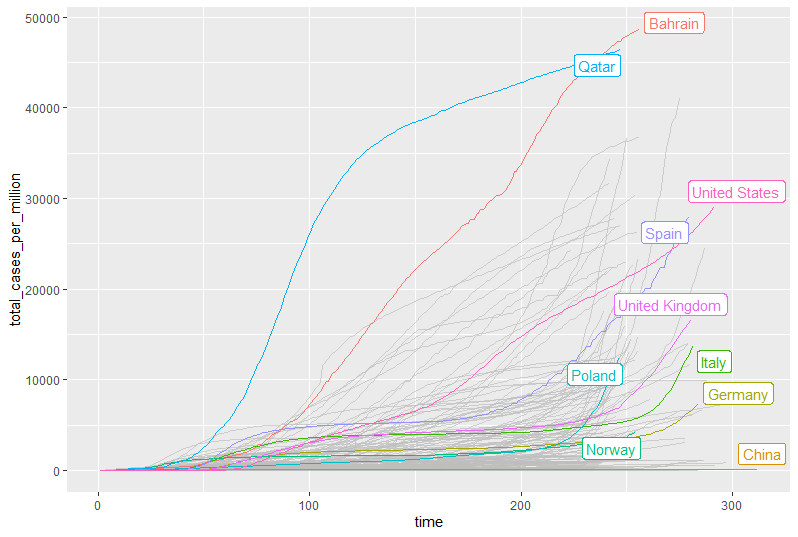
\includegraphics[width=\linewidth]{rys/total_cases_countries.png}
	\caption{Wykres przedstawiający zależność liczby zachorowań na milion mieszkańców w zależności od czasu z podziałem na kraje}
	\label{fig:total_cases_countries}
	\zrodlo{Opracowanie własne}
\end{figure}



Pierwszy model ma postać 

$$y_{total\_cases}=\beta_0 + X_{time}\beta_{time}+Z_{location}u_{location}+\varepsilon$$

a więc przedstawia zależność liczby zachorowań od czasu, a kraj jest efektem losowym.

\newpage




\begin{table}[!htbp]
	\begin{center}
		\begin{tabular}{l c}
			\hline
			& Model 1 \\
			\hline
			(Intercept)               & $-1941.35^{***}$ \\
			& $(337.72)$       \\
			time                      & $37.31^{***}$    \\
			& $(0.26)$         \\
			\hline
			AIC                       & $806648.05$      \\
			BIC                       & $806682.57$      \\
			Log Likelihood            & $-403320.03$     \\
			Num. obs.                 & $41287$          \\
			Num. groups: location     & $151$            \\
			Var: location (Intercept) & $16967251.36$    \\
			Var: Residual             & $17530563.89$    \\
			\hline
			\multicolumn{2}{l}{\scriptsize{$^{***}p<0.001$; $^{**}p<0.01$; $^{*}p<0.05$}}
		\end{tabular}
		\caption{Wyniki dla modelu 1}
		\label{table:model1}
		\zrodlo{Opracowanie własne}
	\end{center}
\end{table}



Widać, że efekt losowy jest odpowiedzialny za ponad połowę wariancji resztowej. Oznacza to, że zmienność liczby zachorowań dla danego kraju jest ponad dwukrotnie mniejsza niż zmienność liczby zachorowań dla różnych krajów.



Zarówno wyraz wolny, jak i współczynnik przy zmiennej \texttt{time}, są istotne statystycznie. Dodatkowo, korelacja pomiędzy liczbą zachorowań a czasem jest dodatnia, więc wraz z upływem czasu liczba zachorowań rośnie.

\newpage

\begin{figure}[htbp]
	\centering
	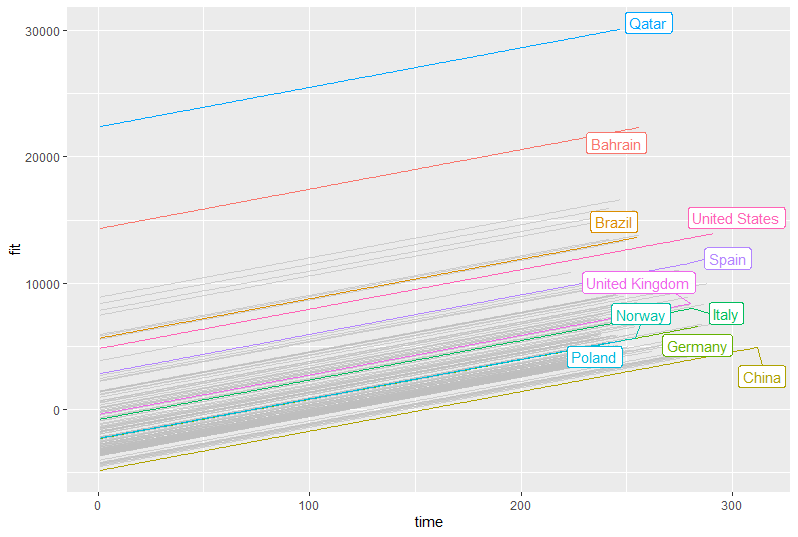
\includegraphics[width=\linewidth]{rys/mod1_predict.png}
	\caption{Wykres przedstawiający zależność między liczbą zachorowań a czasem oszacowaną za pomocą Modelu 1}
	\label{fig:mod1_predict}
	\zrodlo{Opracowanie własne}
\end{figure}

Na rysunku \ref{fig:mod1_predict} widzimy linie dopasowane do liczby zachorowań w porzczególnych krajach. Każda prosta ma taki sam współczynnik kierunkowy, jedynie punkt przecięcia z osią OY (\texttt{Intercept}) różni się pomiędzy poszczególnymi krajami. Z tego wykresu możemy odczytać, jak różnią się średnie poziomy liczby zachorowań między krajami.

\newpage

Oprócz powyższego modelu, w którym tylko wyraz wolny różni się pomiędzy krajami, można rozważyć także model, gdzie współczynnik nachylenia prostej także będzie zależał od efektu losowego, czyli model postaci:

$$y_{total\_cases}=\beta_0+X_{time}\beta_{time}+Z_{0,location}u_{0,location}+$$$$+Z_{time,location}u_{time,location}+\varepsilon$$

\begin{table}[!htbp]
	\begin{center}
		\begin{tabular}{l c}
			\hline
			& Model 1 \\
			\hline
			(Intercept)                    & $-1784.78^{***}$ \\
			& $(145.44)$       \\
			time                           & $35.49^{***}$    \\
			& $(2.93)$         \\
			\hline
			AIC                            & $759067.36$      \\
			BIC                            & $759119.13$      \\
			Log Likelihood                 & $-379527.68$     \\
			Num. obs.                      & $41287$          \\
			Num. groups: location          & $151$            \\
			Var: location (Intercept)      & $3113329.04$     \\
			Var: location time             & $1296.95$        \\
			Cov: location (Intercept) time & $-53442.24$      \\
			Var: Residual                  & $5450792.56$     \\
			\hline
			\multicolumn{2}{l}{\scriptsize{$^{***}p<0.001$; $^{**}p<0.01$; $^{*}p<0.05$}}
		\end{tabular}
		\caption{Wyniki dla modelu 1}
		\label{table:model1-1}
		\zrodlo{Opracowanie własne}
	\end{center}
\end{table}

\newpage

\begin{figure}[htbp]
	\centering
	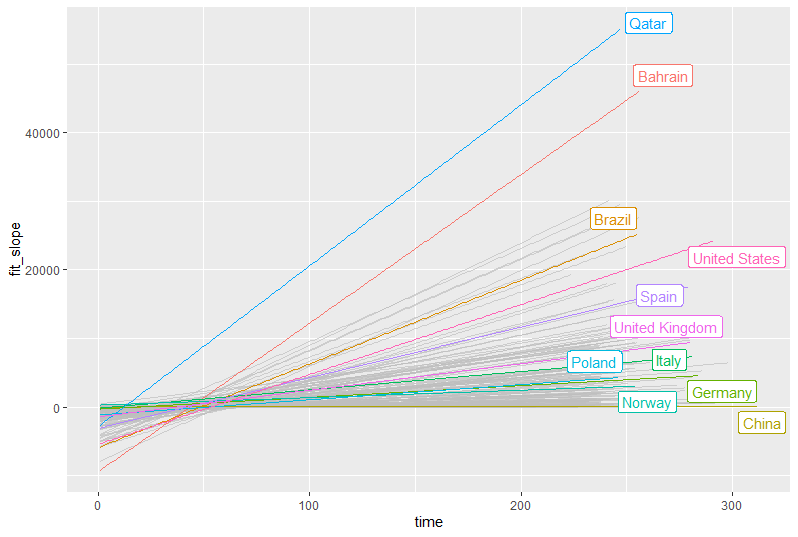
\includegraphics[width=\linewidth]{rys/mod1_slope_predict.png}
	\caption{Wykres przedstawiający zależność między liczbą zachorowań a czasem oszacowaną za pomocą modelu, gdzie zarówno wyraz wolny, jak i współczynnik nachylenia prostej różnią się pomiędzy krajami}
	\label{fig:mod1_slope_predict}
	\zrodlo{Opracowanie własne}
\end{figure}

Na rysunku \ref{fig:mod1_slope_predict} można zaobserwować, jak różnią się tendencje rozwojowe pandemii w poszczególnych krajach.

\newpage

W analogiczny sposób można zbudować model, gdzie zależność od czasu będzie funkcją kwadratową, to jest

$$y_{total\_cases}=\beta_0+X_{time}\beta_{time}+X_{time^2}\beta_{time^2}+$$$$+Z_{0,location}u_{0,location}+Z_{time,location}u_{time,location}+$$$$Z_{time^2,location}u_{time^2, location}+\varepsilon$$

\begin{table}[!htbp]
	\begin{center}
		\begin{tabular}{l c}
			\hline
			& Model 1 \\
			\hline
			(Intercept)                           & $383.14^{***}$ \\
			& $(107.34)$     \\
			time                                  & $-10.66$       \\
			& $(161.66)$     \\
			time$^2$                              & $0.16$         \\
			& $(0.21)$       \\
			\hline
			AIC                                   & $721041.58$    \\
			BIC                                   & $721127.86$    \\
			Log Likelihood                        & $-360510.79$   \\
			Num. obs.                             & $41287$        \\
			Num. groups: location                 & $151$          \\
			Var: location (Intercept)             & $1671050.31$   \\
			Var: location time                    & $3946212.95$   \\
			Var: location I(time$^2$)             & $6.52$         \\
			Cov: location (Intercept) time        & $24812.00$     \\
			Cov: location (Intercept) I(time$^2$) & $279.78$       \\
			Cov: location time I(time$^2$)        & $5030.38$      \\
			Var: Residual                         & $2045067.48$   \\
			\hline
			\multicolumn{2}{l}{\scriptsize{$^{***}p<0.001$; $^{**}p<0.01$; $^{*}p<0.05$}}
		\end{tabular}
		\caption{Wyniki dla modelu 1 z czynnikiem kwadratowym}
		\label{table:model1-2}
		\zrodlo{Opracowanie własne}
	\end{center}
\end{table}

Po dodaniu do modelu drugiej potęgi zmiennej $time$, wpływ czasu przestaje być istotny.

\begin{figure}[htbp]
	\centering
	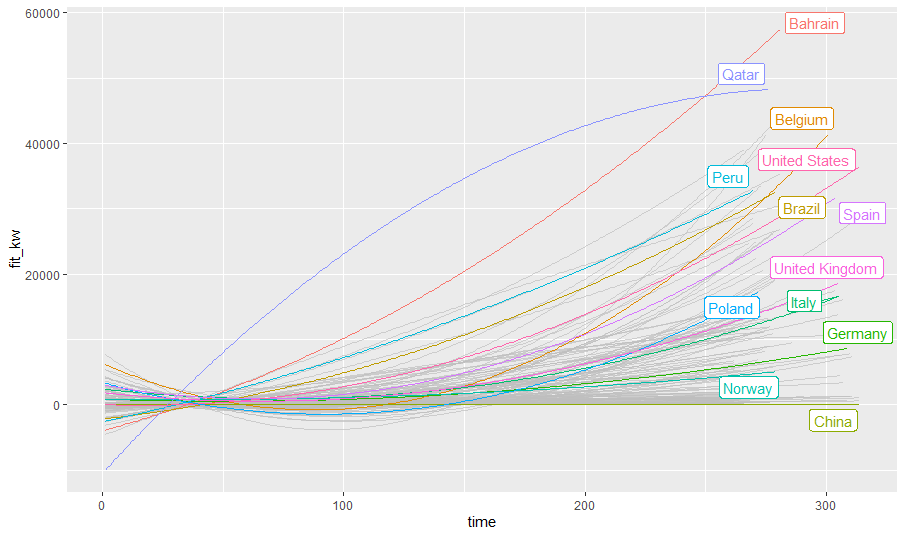
\includegraphics[width=\linewidth]{rys/mod1_kw_predict.png}
	\caption{Wykres przedstawiający zależność między liczbą zachorowań a czasem oszacowaną za pomocą modelu, gdzie zarówno wyraz wolny, jak i współczynniki przy $time$ i $time^2$ zależą od kraju}
	\label{fig:mod1_kw_predict}
	\zrodlo{Opracowanie własne}
\end{figure}

\newpage

\subsection{Model 2}

Hipoteza 2: Liczba wykonywanych testów na COVID-19 ma związek z liczbą zachorowań.

\newpage

\begin{figure}[htbp]
	\centering
	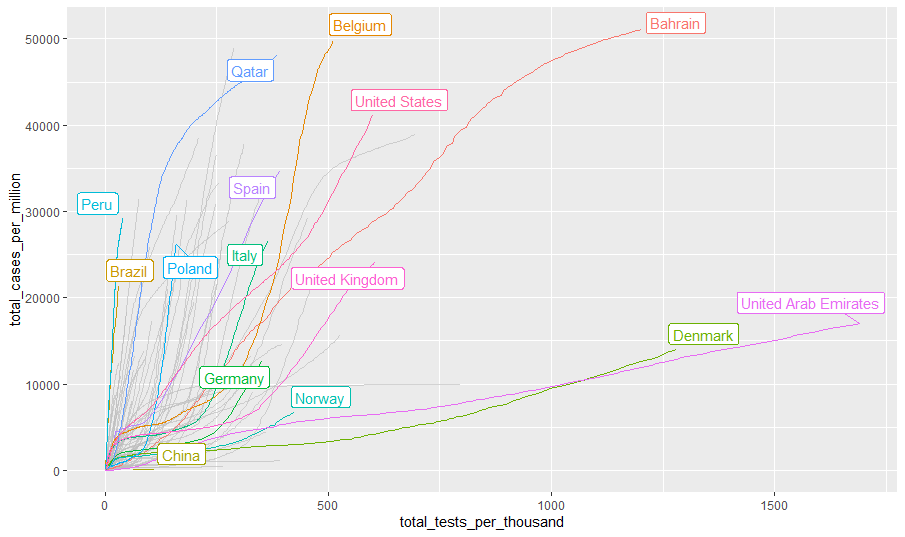
\includegraphics[width=\linewidth]{rys/total_tests_countries.png}
	\caption{Wykres przedstawiający zależność między liczbą zachorowań a liczbą wykonywanych testów w poszczególnych krajach}
	\label{fig:tests}
	\zrodlo{Opracowanie własne}
\end{figure}

Drugi model to:

$$y_{total\_ cases}=\beta_0 + X_{total\_tests}\beta_{total\_ tests}+Z_{location}u_{location}+\varepsilon$$

Badamy tutaj, czy liczba wykonywanych testów (w przeliczeniu na 1000 mieszkańców) ma wpływ na liczbę zachorowań.

Dla tego modelu otrzymujemy następujące wyniki:
\newpage
\begin{table}[!htbp]
	\begin{center}
		\begin{tabular}{l c}
			\hline
			& Model 1 \\
			\hline
			(Intercept)                 & $1741.18^{***}$ \\
			& $(464.57)$      \\
			total\_tests\_per\_thousand & $34.85^{***}$   \\
			& $(0.28)$        \\
			\hline
			AIC                         & $430649.03$     \\
			BIC                         & $430681.01$     \\
			Log Likelihood              & $-215320.52$    \\
			Num. obs.                   & $21907$         \\
			Num. groups: location       & $97$            \\
			Var: location (Intercept)   & $20699413.62$   \\
			Var: Residual               & $19714018.35$   \\
			\hline
			\multicolumn{2}{l}{\scriptsize{$^{***}p<0.001$; $^{**}p<0.01$; $^{*}p<0.05$}}
		\end{tabular}
		\caption{Wyniki dla modelu 2}
		\label{table:model2}
		\zrodlo{Opracowanie własne}
	\end{center}
\end{table}

Widać po pierwsze, że efekt losowy jest odpowiedzialny za ponad połowę zmienności resztowej modelu. Po drugie, widać, że efekt stały liczby wykonywanych testów jest istotny statystycznie, i ma wpływ stymulujący na liczbę zachorowań.

\newpage

\begin{figure}[htbp]
	\centering
	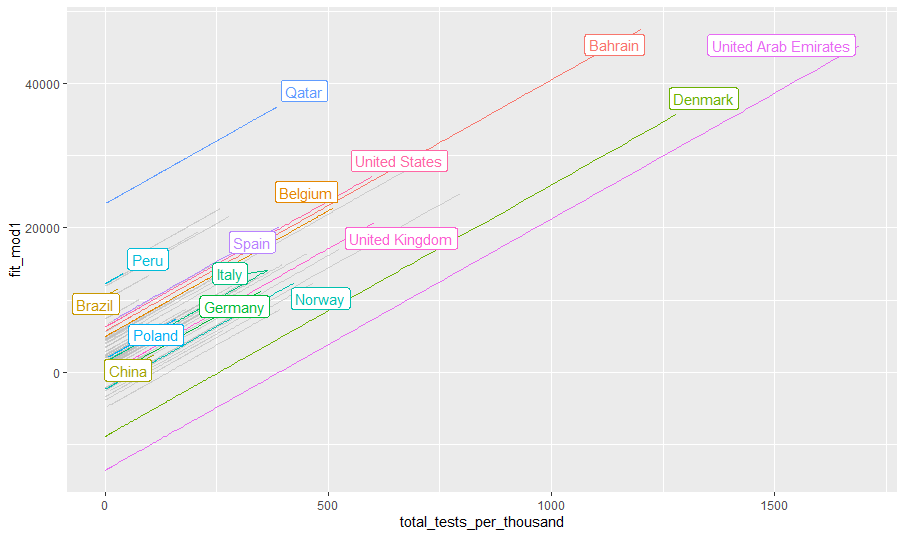
\includegraphics[width=\linewidth]{rys/mod2_predict.png}
	\caption{Wykres przedstawiający dopasowanie modelu random intercept}
	\label{fig:mod2}
	\zrodlo{Opracowanie własne}
\end{figure}



Można także dopasować model, w którym współczynnik nachylenia prostej zależy od kraju:

$$y_{total\_ cases}=\beta_0 + X_{total\_tests}\beta_{total\_ tests}+$$
$$+Z_{0,location}u_{0,location}+Z_{total\_tests, location}u_{total\_tests, location}+\varepsilon$$
\newpage
\begin{table}[!htbp]
\begin{center}
	\begin{tabular}{l c}
		\hline
		& Model 1 \\
		\hline
		(Intercept)                                           & $-324.65$      \\
		& $(175.92)$     \\
		total\_tests\_per\_thousand                           & $109.17^{***}$ \\
		& $(13.83)$      \\
		\hline
		AIC                                                   & $391507.90$    \\
		BIC                                                   & $391555.87$    \\
		Log Likelihood                                        & $-195747.95$   \\
		Num. obs.                                             & $21907$        \\
		Num. groups: location                                 & $97$           \\
		Var: location (Intercept)                             & $2910697.88$   \\
		Var: location total\_tests\_per\_thousand             & $18059.27$     \\
		Cov: location (Intercept) total\_tests\_per\_thousand & $-6245.44$     \\
		Var: Residual                                         & $3206479.62$   \\
		\hline
		\multicolumn{2}{l}{\scriptsize{$^{***}p<0.001$; $^{**}p<0.01$; $^{*}p<0.05$}}
	\end{tabular}
	\caption{Wyniki dla modelu 2 z losowym współczynnikiem nachylenia}
	\label{table:mod2-1}
\end{center}
\end{table}

\newpage

\begin{figure}[htbp]
	\centering
	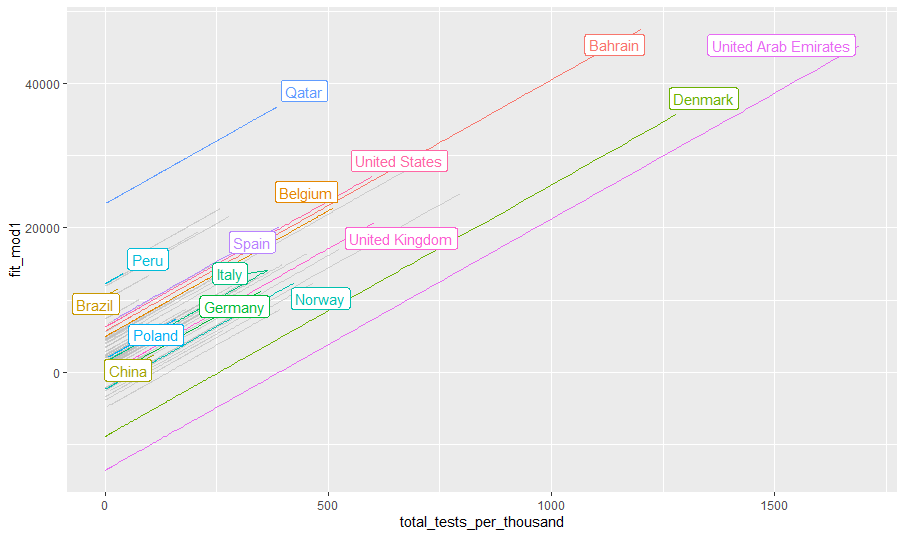
\includegraphics[width=\linewidth]{rys/mod2_predict.png}
	\caption{Wykres przedstawiający dopasowanie modelu random intercept and slope}
	\label{fig:mod2-slope}
	\zrodlo{Opracowanie własne}
\end{figure}

\newpage


\subsection{Model 3}


Hipoteza 3: kraje o różnej oczekiwanej długości życia różnią się liczbą zachorowań.

Trzeci model jest modelem liniowym:

$$y_{total\_cases}=\beta_0+X_{life\_expectancy}\beta_{life\_expectancy}+\varepsilon$$

Prezentuje on zależność liczby zachorowań od oczekiwanej długości życia w danym kraju.

Dla modelu trzeciego otrzymujemy następujące wyniki:

\begin{table}[!htbp]
	\begin{center}
		\begin{tabular}{l c}
			\hline
			& Model 1 \\
			\hline
			(Intercept)      & $-14780.85^{***}$ \\
			& $(294.55)$        \\
			life\_expectancy & $248.30^{***}$    \\
			& $(4.03)$          \\
			\hline
			R$^2$            & $0.08$            \\
			Adj. R$^2$       & $0.08$            \\
			Num. obs.        & $41287$           \\
			\hline
			\multicolumn{2}{l}{\scriptsize{$^{***}p<0.001$; $^{**}p<0.01$; $^{*}p<0.05$}}
		\end{tabular}
		\caption{Wyniki dla modelu 3}
		\label{table:model3}
		\zrodlo{Opracowanie własne}
	\end{center}
\end{table}
\newpage
\begin{figure}[htbp]
	\centering
	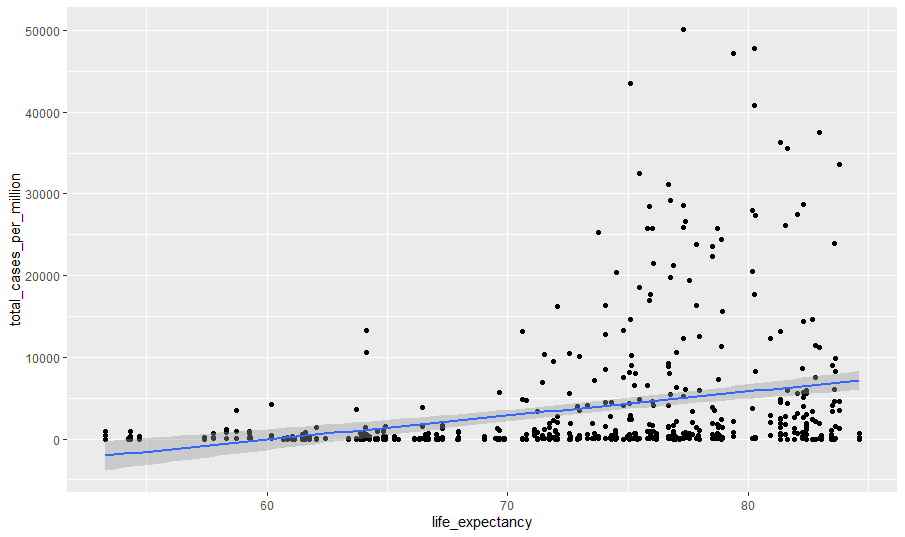
\includegraphics[width=\linewidth]{rys/mod3-lin.png}
	\caption{Wykres przedstawiający dopasowanie modelu liniowego bez przekształcenia zmiennych}
	\label{fig:mod3-lin}
	\zrodlo{Opracowanie własne}
\end{figure}

Z analizy modelu liniowego wynika, że oczekiwana długość życia ma istotny wpływ na liczbę zachorowań. Im większa jest oczekiwana długość życia, tym więcej będzie potwierdzonych przypadków koronawirusa. Z wykresu oraz na podstawie niskiej wartości $R^2$ (około 8\%) wynika, że model jest słabo dopasowany do danych. Można zastosować transformację zmiennych, aby poprawić dopasowanie.

Z transformacji Boxa-Coxa otrzymujemy następujące potęgi dla zmiennych: $3.72$ dla life\_expectancy oraz $0.09$ dla total\_cases\_per\_million. W przybliżeniu przyjmiemy czwartą potęgę dla pierwszej cechy, a dla drugiej 0 czyli logarytm.

$$log(y_{total\_cases})=\beta_0+\beta_{life\_expectancy}X_{life\_expectancy}^4+\varepsilon$$
\newpage
\begin{table}[!htbp]
	\begin{center}
		\begin{tabular}{l c}
		\hline
		& Model 1 \\
		\hline
		(Intercept)          & $3.22^{***}$ \\
		& $(0.04)$     \\
		life\_expectancy$^4$ & $0.00^{***}$ \\
		& $(0.00)$     \\
		\hline
		R$^2$                & $0.10$       \\
		Adj. R$^2$           & $0.10$       \\
		Num. obs.            & $41287$      \\
		\hline
		\multicolumn{2}{l}{\scriptsize{$^{***}p<0.001$; $^{**}p<0.01$; $^{*}p<0.05$}}
	\end{tabular}
		\caption{Wyniki dla modelu 3 po przekształceniu zmiennych}
		\label{table:mod3-potega}
	\end{center}
\end{table}

\begin{figure}[htbp]
	\centering
	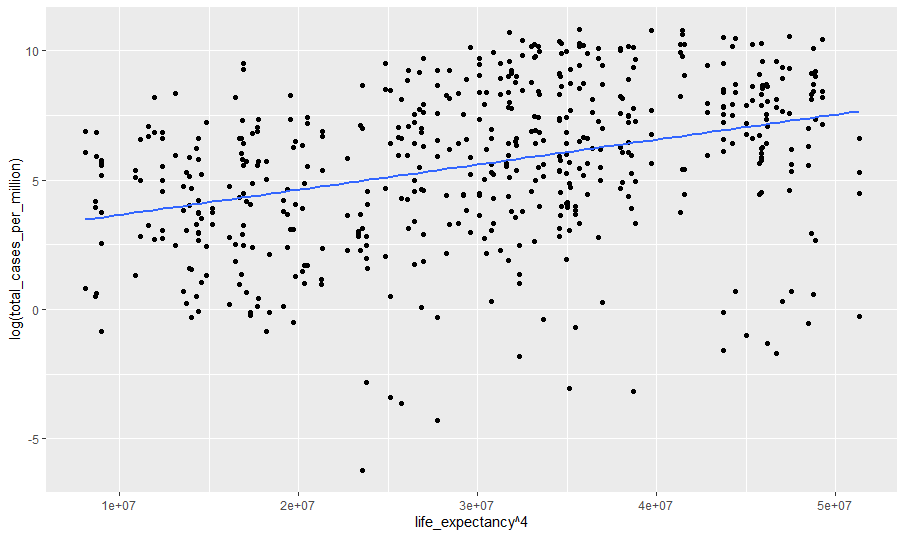
\includegraphics[width=\linewidth]{rys/mod3-potega.png}
	\caption{Wykres przedstawiający dopasowanie modelu liniowego z przekształceniem zmiennych}
	\label{fig:mod3-potega}
	\zrodlo{Opracowanie własne}
\end{figure}




	


Po przekształceniu, $R^2$ wzrosło nieznacznie, do 10\%. Wniosek pozostaje ten sam - im wyższa oczekiwana długość życia, tym więcej osób chorych na COVID-19.

\newpage

\subsection{Model 4}

Hipoteza 4: Kraje o różnej gęstości zaludnienia różnią się liczbą zachorowań.

W czwartym modelu badamy zależnośc liczby zachorowań od gęstości zaludnienia:

$$y_{total\_cases}=\beta_0+X_{population\_density}\beta_{population\_density}+\varepsilon$$


Wyniki są następujące:

\begin{table}[!htbp]
	\begin{center}
		\begin{tabular}{l c}
			\hline
			& Model 1 \\
			\hline
			(Intercept)         & $3606.05^{***}$ \\
			& $(356.36)$      \\
			population\_density & $0.64$          \\
			& $(0.49)$        \\
			\hline
			R$^2$               & $0.00$          \\
			Adj. R$^2$          & $0.00$          \\
			Num. obs.           & $537$           \\
			\hline
			\multicolumn{2}{l}{\scriptsize{$^{***}p<0.001$; $^{**}p<0.01$; $^{*}p<0.05$}}
		\end{tabular}
		\caption{Wyniki dla modelu 4}
		\label{table:mod4}
	\end{center}
\end{table}

Gęstośc zaludnienia nie jest czynnikiem istotnym statystycznie, a $R^2$ wynosi 0. Zatem liczba zachorowań na COVID-19 nie zależy od gęstości zaludnienia.

\begin{figure}[htbp]
	\centering
	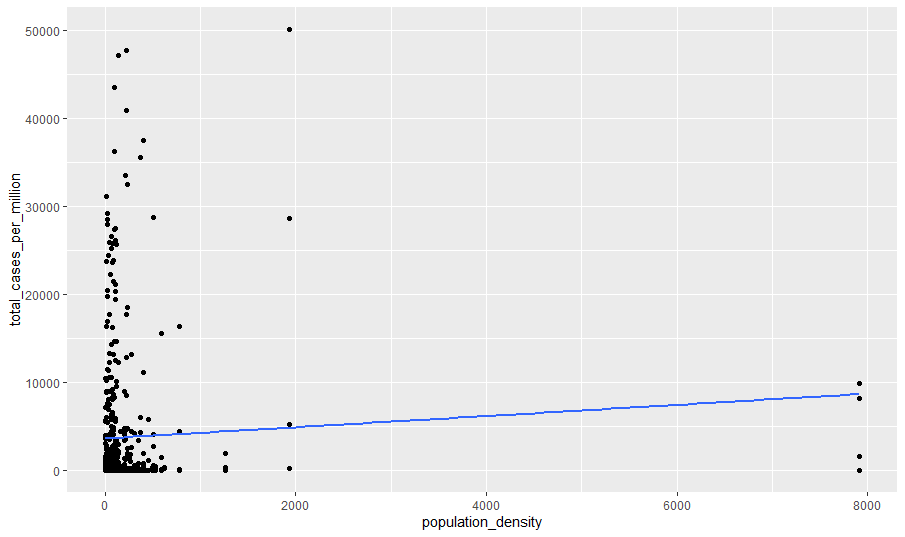
\includegraphics[width=\linewidth]{rys/mod4-lin.png}
	\caption{Wykres przedstawiający dopasowanie modelu liniowego }
	\label{fig:mod4-lin}
	\zrodlo{Opracowanie własne}
\end{figure}

\newpage

\subsection{Model 5}

Hipoteza 5: Kraje różniące się siłą obostrzeń mają istotne różnice w liczbie zachorowań.
\newpage
\begin{figure}[htbp]
	\centering
	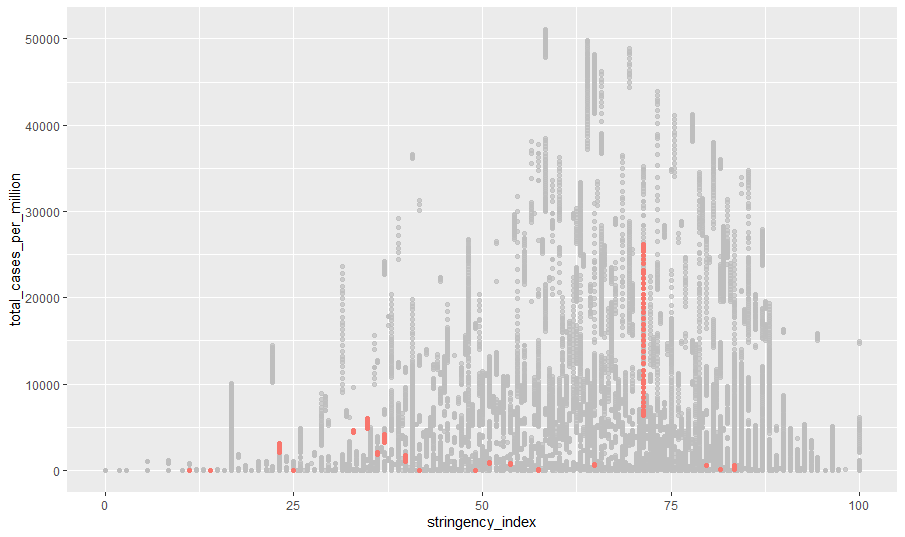
\includegraphics[width=\linewidth]{rys/stringency_pol.png}
	\caption{Wykres przedstawiający zależność liczby zachorowań od współczynnika siły obostrzeń, kolorem zaznaczone dane dla Polski}
	\label{fig:stringency-pol}
	\zrodlo{Opracowanie własne}
\end{figure}

Piąty model ma następującą postać:

$$y_{total\_cases}=\beta_0+X_{stringency\_index}\beta_{stringency\_index}+Z_{location}u_{location}+\varepsilon$$

W tym modelu sprawdzamy zależność liczby zachorowań od siły obostrzeń.
\newpage
Otrzymujemy następujące wyniki:

\begin{table}[!htbp]
	\begin{center}
		\begin{tabular}{l c}
			\hline
			& Model 1 \\
			\hline
			(Intercept)               & $3319.47^{***}$ \\
			& $(356.25)$      \\
			stringency\_index         & $-3.27^{*}$     \\
			& $(1.43)$        \\
			\hline
			AIC                       & $801139.90$     \\
			BIC                       & $801174.31$     \\
			Log Likelihood            & $-400565.95$    \\
			Num. obs.                 & $40219$         \\
			Num. groups: location     & $147$           \\
			Var: location (Intercept) & $17448313.08$   \\
			Var: Residual             & $25718203.07$   \\
			\hline
			\multicolumn{2}{l}{\scriptsize{$^{***}p<0.001$; $^{**}p<0.01$; $^{*}p<0.05$}}
		\end{tabular}
		\caption{Wyniki dla modelu 5}
		\label{table:model5}
		\zrodlo{Opracowanie własne}
	\end{center}
\end{table}
Wskaźnik siły obostrzeń jest istotny statystycznie i ma wpływ ograniczający, co oznacza, że im silniejsze obostrzenia, tym mniejsza liczba zachorowań w danym kraju.

\begin{figure}[htbp]
	\centering
	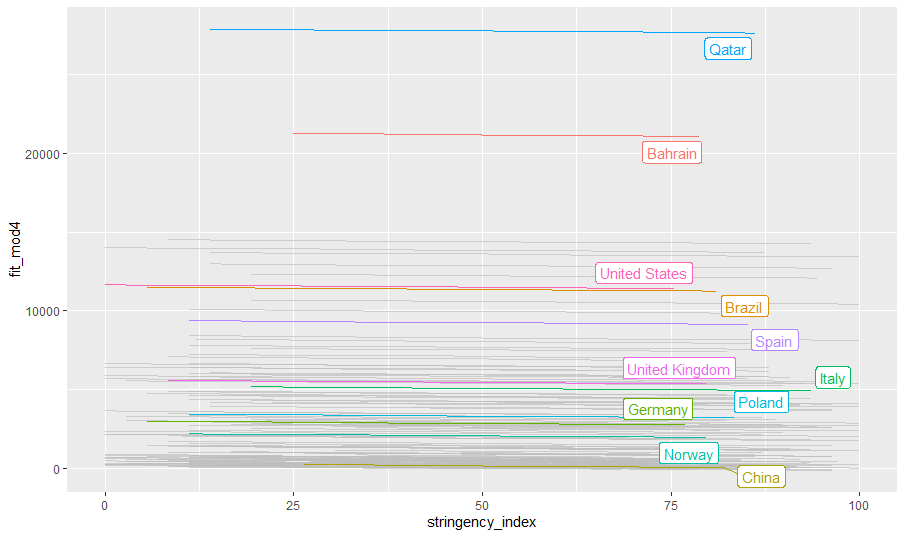
\includegraphics[width=\linewidth]{rys/mod5_predict.png}
	\caption{Wykres przedstawiający dopasowanie modelu random intercept}
	\label{fig:mod5_predict}
	\zrodlo{Opracowanie własne}
\end{figure}


\begin{table}[!htbp]
	\begin{center}
		\begin{tabular}{l c}
			\hline
			& Model 1 \\
			\hline
			(Intercept)                                 & $4607.01^{***}$ \\
			& $(711.39)$      \\
			stringency\_index                           & $-15.60$        \\
			& $(8.46)$        \\
			\hline
			AIC                                         & $797733.02$     \\
			BIC                                         & $797784.63$     \\
			Log Likelihood                              & $-398860.51$    \\
			Num. obs.                                   & $40219$         \\
			Num. groups: location                       & $147$           \\
			Var: location (Intercept)                   & $71934195.57$   \\
			Var: location stringency\_index             & $9970.86$       \\
			Cov: location (Intercept) stringency\_index & $-699926.27$    \\
			Var: Residual                               & $23308070.03$   \\
			\hline
			\multicolumn{2}{l}{\scriptsize{$^{***}p<0.001$; $^{**}p<0.01$; $^{*}p<0.05$}}
		\end{tabular}
		\caption{Wyniki dla modelu 5 z losowym współczynnikiem nachylenia}
		\label{table:mod5-slope}
	\end{center}
\end{table}

\begin{figure}[htbp]
	\centering
	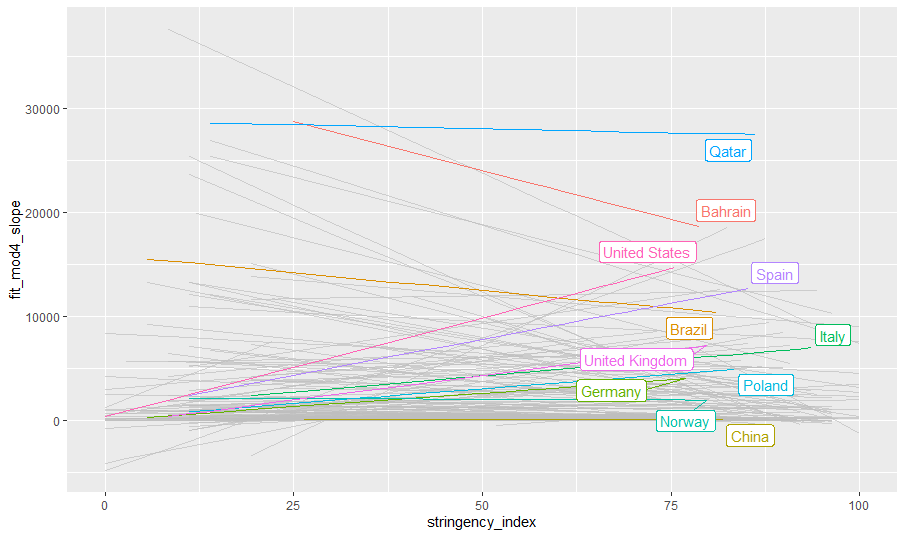
\includegraphics[width=\linewidth]{rys/mod5_predict_slope.png}
	\caption{Wykres przedstawiający dopasowanie modelu random intercept and slope}
	\label{fig:mod5_predict_slope}
	\zrodlo{Opracowanie własne}
\end{figure}

Z wykresu \ref{fig:mod5_predict_slope} widać, że w niektórych krajach przy wzroście siły obostrzeń, liczba zachorowań maleje, a w innych rośnie. Dla przeciętnego kraju wpływ jest ograniczający (co wynika z tabeli \ref{table:mod5-slope}).

\newpage

\subsection{Model 6}

Hipoteza 6: Kraje o różnej wysokości wskaźnika rozwoju społecznego (HDI) różnią się liczbą zachorowań.

Szósty model przedstawia zależność liczby zachorowań od wskaźnika rozwoju społecznego:

$$y_{total\_cases}=\beta_0+X_{HDI}\beta_{HDI}+\varepsilon$$

Z tego modelu mamy następujący wynik:

\begin{table}[!htbp]
	\begin{center}
		\begin{tabular}{l c}
			\hline
			& Model 1 \\
			\hline
			(Intercept)               & $-5916.47^{***}$ \\
			& $(145.15)$       \\
			human\_development\_index & $12894.77^{***}$ \\
			& $(198.99)$       \\
			\hline
			R$^2$                     & $0.09$           \\
			Adj. R$^2$                & $0.09$           \\
			Num. obs.                 & $41027$          \\
			\hline
			\multicolumn{2}{l}{\scriptsize{$^{***}p<0.001$; $^{**}p<0.01$; $^{*}p<0.05$}}
		\end{tabular}
		\caption{Wyniki dla modelu 6}
		\label{table:mod6}
	\end{center}
\end{table}

HDI jest istotny i ma wpływ stymulujacy. W krajach z wyższym wskaźnikiem rozwoju społecznego, zachorowań jest znacząco więcej.

\begin{figure}[htbp]
	\centering
	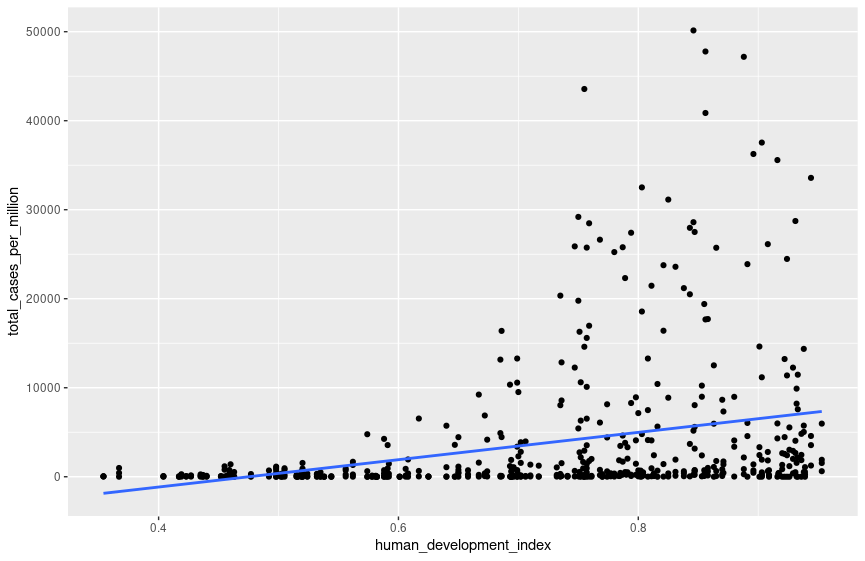
\includegraphics[width=\linewidth]{rys/mod6-lin.png}
	\caption{Wykres przedstawiający dopasowanie modelu liniowego}
	\label{fig:mod6-lin}
	\zrodlo{Opracowanie własne}
\end{figure}
\newpage
Z przekształcenia Boxa-Coxa otrzymujemy potęgę 2 dla zmiennej HDI oraz 0 dla total\_cases.

\begin{table}[!htbp]
	\begin{center}
		\begin{tabular}{l c}
			\hline
			& Model 1 \\
			\hline
			(Intercept)                   & $3.11^{***}$ \\
			& $(0.04)$     \\
			human\_development\_index$^2$ & $4.98^{***}$ \\
			& $(0.07)$     \\
			\hline
			R$^2$                         & $0.12$       \\
			Adj. R$^2$                    & $0.12$       \\
			Num. obs.                     & $41027$      \\
			\hline
			\multicolumn{2}{l}{\scriptsize{$^{***}p<0.001$; $^{**}p<0.01$; $^{*}p<0.05$}}
		\end{tabular}
		\caption{Wyniki dla modelu 6 po przekształceniu zmiennych}
		\label{table:mod6-log}
	\end{center}
\end{table}
\newpage
\begin{figure}[htbp]
	\centering
	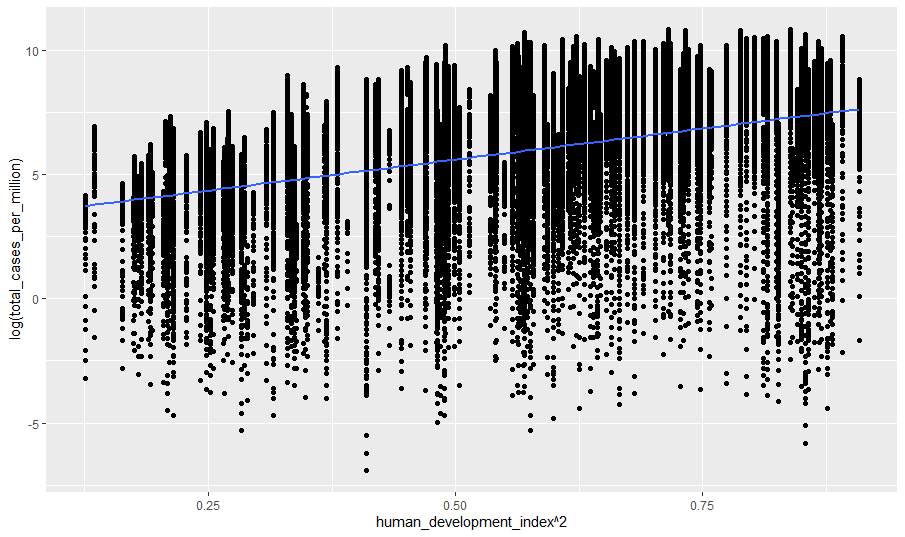
\includegraphics[width=\linewidth]{rys/mod6-log.png}
	\caption{Wykres przedstawiający dopasowanie modelu liniowego z przekształceniem zmiennych}
	\label{fig:mod6-log}
	\zrodlo{Opracowanie własne}
\end{figure}

\newpage

\subsection{Model 7}

Hipoteza 7: Kraje o różnej wysokości odsetka śmierci z powodu chorób sercowych różnią się liczbą zachorowań.

Model siódmy wygląda następująco:

$$y_{total\_cases}=\beta_0+X_{cardiovasc\_death\_rate}\beta_{cardiovasc\_death\_rate}+\varepsilon$$

i zawiera zależność od odsetka śmierci spowodowanych chorobami sercowymi w danym kraju. 

Otrzymujemy następujące podsumowanie:

\begin{table}[!htbp]
	\begin{center}
		\begin{tabular}{l c}
			\hline
			& Model 1 \\
			\hline
			(Intercept)             & $6602.10^{***}$ \\
			& $(792.12)$      \\
			cardiovasc\_death\_rate & $-11.06^{***}$  \\
			& $(2.76)$        \\
			\hline
			R$^2$                   & $0.03$          \\
			Adj. R$^2$              & $0.03$          \\
			Num. obs.               & $537$           \\
			\hline
			\multicolumn{2}{l}{\scriptsize{$^{***}p<0.001$; $^{**}p<0.01$; $^{*}p<0.05$}}
		\end{tabular}
		\caption{Wyniki dla modelu 7}
		\label{table:model7}
		\zrodlo{Opracowanie własne}
	\end{center}
\end{table}
\newpage
\begin{figure}[htbp]
	\centering
	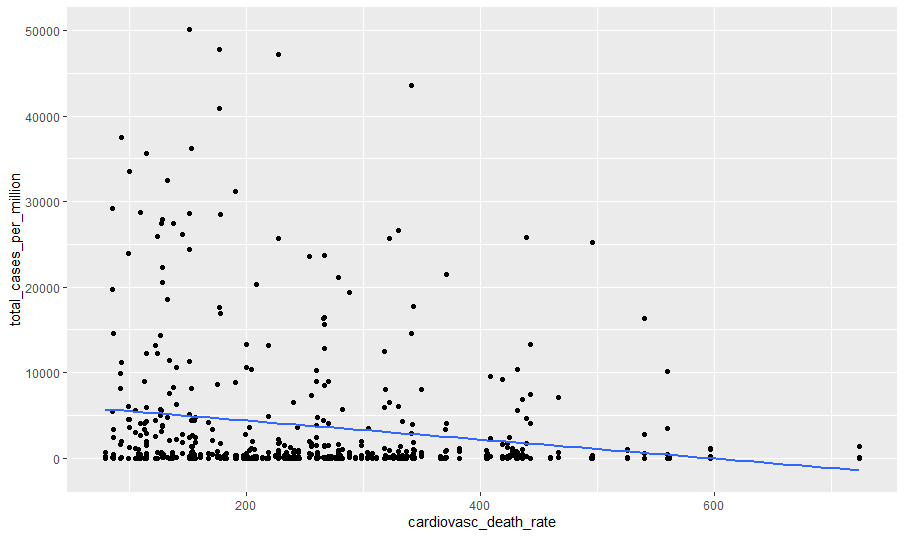
\includegraphics[width=\linewidth]{rys/mod7-lin.png}
	\caption{Wykres przedstawiający dopasowanie modelu liniowego}
	\label{fig:mod7-lin}
	\zrodlo{Opracowanie własne}
\end{figure}

 Efekt śmiertelności na choroby serca jest istotny statystycznie. Co ciekawe, odsetek śmierci spowodowanych chorobami serca wpływa ograniczająco na liczbę zachorowań. Może to być związane z tym, że osoby chore na serce bardziej uważają, aby się nie zarazić, tym samym zmniejszają liczbę zachorowań w danym kraju.

Przekształcenie Boxa-Coxa: pierwiastek 3 stopnia z cardiovasc, log z total cases.

\begin{table}[!htbp]
	\begin{center}
		\begin{tabular}{l c}
			\hline
			& Model 1 \\
			\hline
			(Intercept)                   & $8.81^{***}$  \\
			& $(0.82)$      \\
			cardiovasc\_death\_rate\^~(1/3) & $-0.52^{***}$ \\
			& $(0.13)$      \\
			\hline
			R$^2$                         & $0.03$        \\
			Adj. R$^2$                    & $0.03$        \\
			Num. obs.                     & $537$         \\
			\hline
			\multicolumn{2}{l}{\scriptsize{$^{***}p<0.001$; $^{**}p<0.01$; $^{*}p<0.05$}}
		\end{tabular}
		\caption{Wyniki dla modelu 7 po przekształceniu zmienych}
		\label{table:mod7-log}
	\end{center}
\end{table}
\newpage
\begin{figure}[htbp]
	\centering
	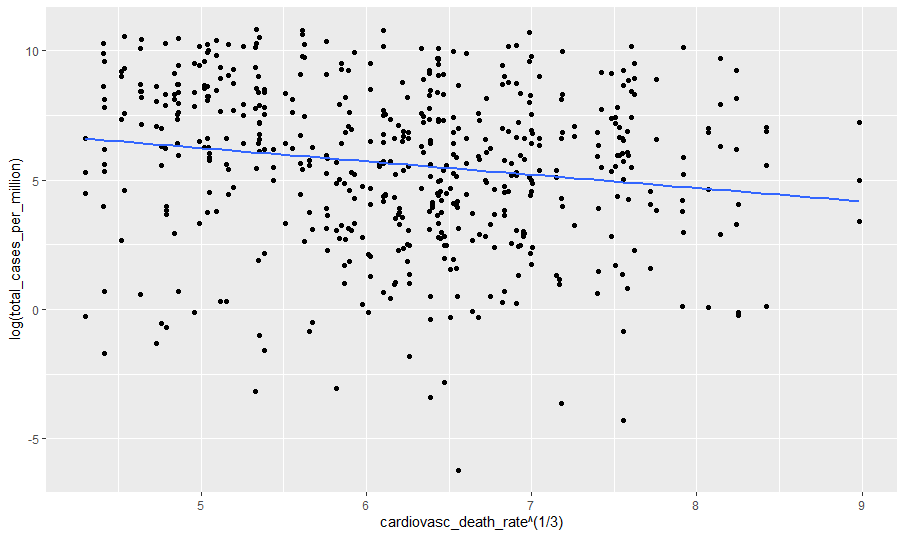
\includegraphics[width=\linewidth]{rys/mod7-log.png}
	\caption{Wykres przedstawiający dopasowanie modelu liniowego po przekształceniu zmiennych}
	\label{fig:mod7-log}
	\zrodlo{Opracowanie własne}
\end{figure}

\newpage

\subsection{Model 8}

Hipoteza 8: Kraje o różnej wysokości odsetka osób chorych na cukrzycę różnią się liczbą zachorowań.

$$y_{total\_cases}=\beta_0+X_{diabetes\_prevalence}\beta_{diabetes\_prevalence}+\varepsilon$$

Model ten jest analogiczny do poprzedniego, z tym że zamiast chorób sercowych mamy tu odsetek chorych na cukrzycę.

Otrzymujemy nastepujący wynik:
\begin{table}[!htbp]
	\begin{center}
\begin{tabular}{l c}
	\hline
	& Model 1 \\
	\hline
	(Intercept)          & $991.31$       \\
	& $(754.70)$     \\
	diabetes\_prevalence & $372.06^{***}$ \\
	& $(91.52)$      \\
	\hline
	R$^2$                & $0.03$         \\
	Adj. R$^2$           & $0.03$         \\
	Num. obs.            & $537$          \\
	\hline
	\multicolumn{2}{l}{\scriptsize{$^{***}p<0.001$; $^{**}p<0.01$; $^{*}p<0.05$}}
\end{tabular}
		\caption{Wyniki dla modelu 8}
		\label{table:model8}
		\zrodlo{Opracowanie własne}
	\end{center}
\end{table}
\newpage
\begin{figure}[htbp]
	\centering
	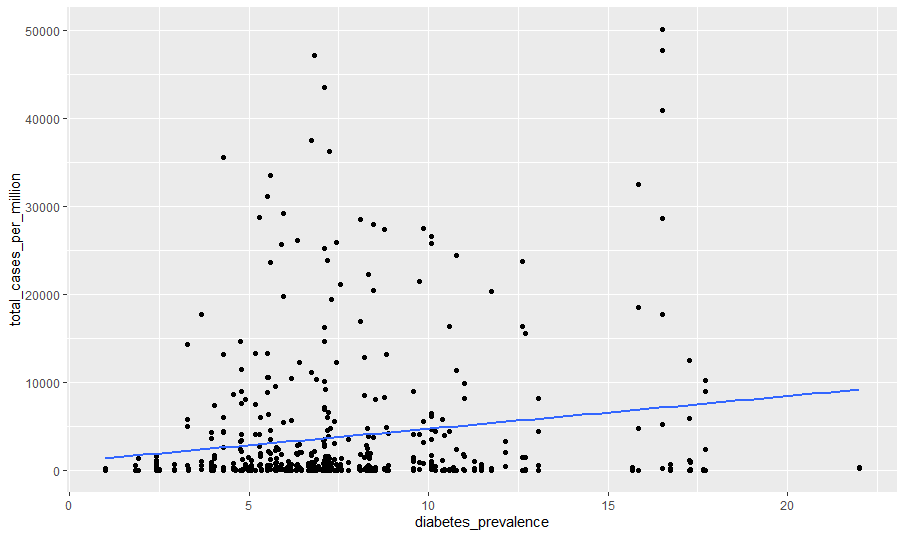
\includegraphics[width=\linewidth]{rys/mod8-lin.png}
	\caption{Wykres przedstawiający dopasowanie modelu liniowego}
	\label{fig:mod8-lin}
	\zrodlo{Opracowanie własne}
\end{figure}

Rozpowszechnienie cukrzycy wpływa stymulująco na liczbę zachorowań. Może to być spowodowane tym, że osoby chore na cukrzycę mają słabszy organizm i są bardziej narażone na zakażenie.



\begin{table}[!htbp]
	\begin{center}
		\begin{tabular}{l c}
			\hline
			& Model 1 \\
			\hline
			(Intercept)                & $2.49^{**}$  \\
			& $(0.79)$     \\
			diabetes\_prevalence\^~(1/3) & $1.65^{***}$ \\
			& $(0.41)$     \\
			\hline
			R$^2$                      & $0.03$       \\
			Adj. R$^2$                 & $0.03$       \\
			Num. obs.                  & $537$        \\
			\hline
			\multicolumn{2}{l}{\scriptsize{$^{***}p<0.001$; $^{**}p<0.01$; $^{*}p<0.05$}}
		\end{tabular}
		\caption{Wyniki dla modelu 8 po przekształceniu zmiennych}
		\label{table:mod8-log}
	\end{center}
\end{table}
\newpage
\begin{figure}[htbp]
	\centering
	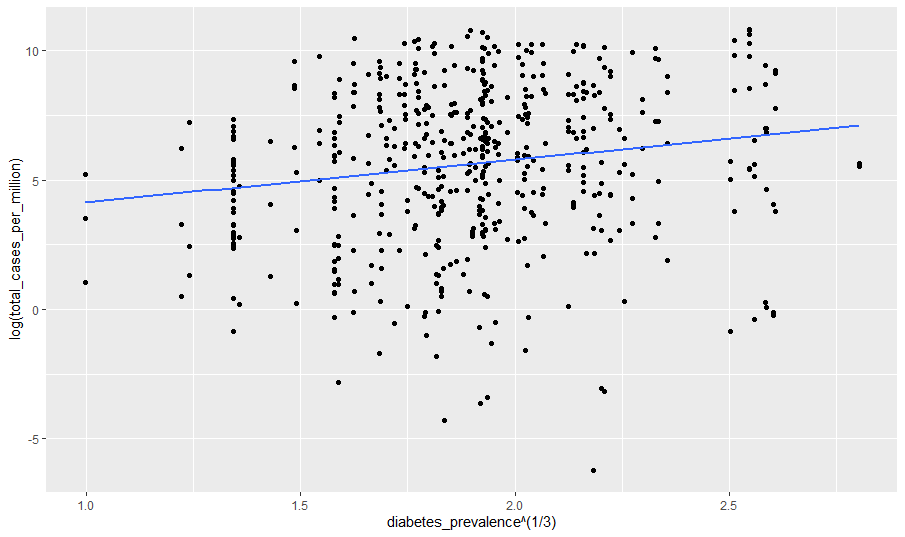
\includegraphics[width=\linewidth]{rys/mod8-log.png}
	\caption{Wykres przedstawiający dopasowanie modelu liniowego z przekształceniem zmiennych}
	\label{fig:mod8-log}
	\zrodlo{Opracowanie własne}
\end{figure}

\newpage

\subsection{Model 9}

Hipoteza 9: Kraje o różnej wysokości odsetka osób żyjących w skrajnej biedzie różnią się liczbą zachorowań.

W tym modelu sprawdzamy zależność liczby zachorowań od odsetka osób żyjących w skrajnym ubóstwie:

$$y_{total\_cases}=\beta_0+X_{extreme\_poverty}\beta_{extreme\_poverty}+\varepsilon$$

Model ten ma następujące podsumowanie:

\begin{table}[!htbp]
	\begin{center}
		\begin{tabular}{l c}
			\hline
			& Model 1 \\
			\hline
			(Intercept)      & $4433.28^{***}$ \\
			& $(406.29)$      \\
			extreme\_poverty & $-83.75^{***}$  \\
			& $(17.02)$       \\
			\hline
			R$^2$            & $0.06$          \\
			Adj. R$^2$       & $0.06$          \\
			Num. obs.        & $389$           \\
			\hline
			\multicolumn{2}{l}{\scriptsize{$^{***}p<0.001$; $^{**}p<0.01$; $^{*}p<0.05$}}
		\end{tabular}
		\caption{Wyniki dla modelu 9}
		\label{table:model9}
		\zrodlo{Opracowanie własne}
	\end{center}
\end{table}

\newpage
\begin{figure}[htbp]
	\centering
	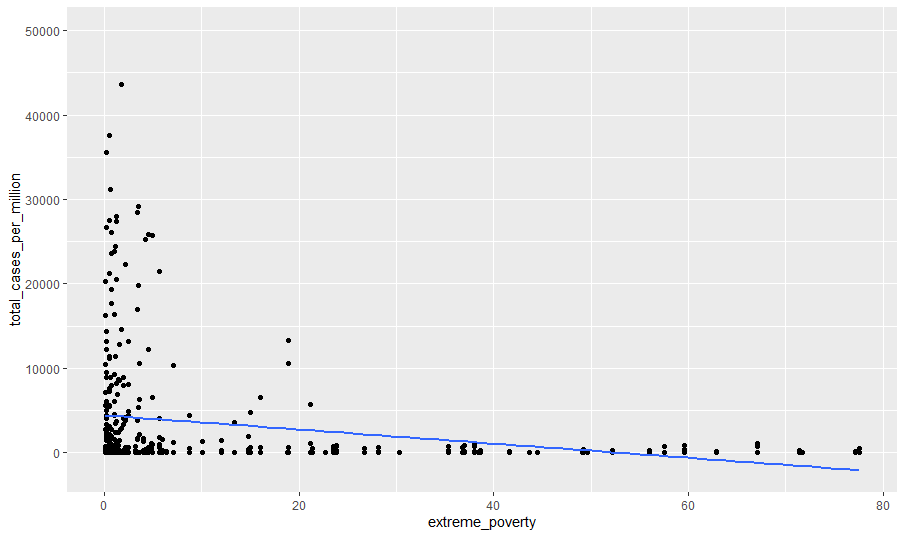
\includegraphics[width=\linewidth]{rys/mod9-lin.png}
	\caption{Wykres przedstawiający dopasowanie modelu liniowego}
	\label{fig:mod9-lin}
	\zrodlo{Opracowanie własne}
\end{figure}

 Czynnik extreme poverty jest istotny statystycznie. Im większy jest w danym kraju odsetek osób żyjących w biedzie, tym niższa liczba zachorowań. Prawdopodobnie jest to spowodowane mniejszą dostępnością do służby zdrowia w biedniejszych krajach i mniejszą liczbą wykonywanych testów.


\begin{table}[!htbp]
	\begin{center}
		\begin{tabular}{l c}
			\hline
			& Model 1 \\
			\hline
			(Intercept)           & $6.00^{***}$  \\
			& $(0.16)$      \\
			log(extreme\_poverty) & $-0.46^{***}$ \\
			& $(0.07)$      \\
			\hline
			R$^2$                 & $0.09$        \\
			Adj. R$^2$            & $0.09$        \\
			Num. obs.             & $389$         \\
			\hline
			\multicolumn{2}{l}{\scriptsize{$^{***}p<0.001$; $^{**}p<0.01$; $^{*}p<0.05$}}
		\end{tabular}
		\caption{Wyniki dla modelu 9 z przekształceniem logarytmicznym obu zmiennych}
		\label{table:mod9-log}
	\end{center}
\end{table}
\newpage
\begin{figure}[htbp]
	\centering
	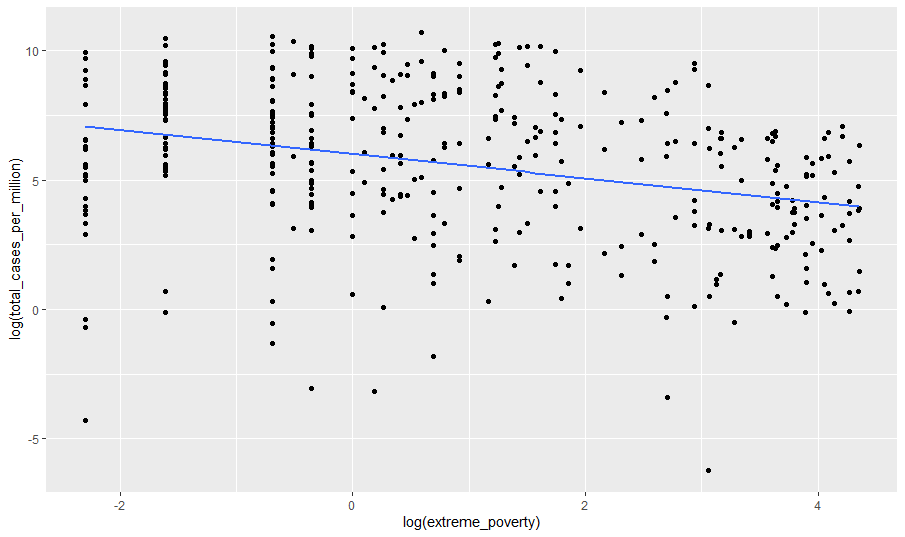
\includegraphics[width=\linewidth]{rys/mod9-log.png}
	\caption{Wykres przedstawiający dopasowanie modelu liniowego z przekształceniem zmiennych}
	\label{fig:mod9-log}
	\zrodlo{Opracowanie własne}
\end{figure}

\newpage

\subsection{Model 10}

Hipoteza 10: Kraje o różnej wysokości PKB różnią się liczbą zachorowań.


W modelu dziesiątym pojawia się zależność liczby zachorowań od PKB na osobę:

$$y_{total\_cases}=\beta_0+X_{GDP}\beta_{GDP}+\varepsilon$$

Wyniki są następujące:
\begin{table}[!htbp]
	\begin{center}
		\begin{tabular}{l c}
			\hline
			& Model 1 \\
			\hline
			(Intercept)      & $1174.04^{*}$ \\
			& $(462.01)$    \\
			gdp\_per\_capita & $0.13^{***}$  \\
			& $(0.02)$      \\
			\hline
			R$^2$            & $0.11$        \\
			Adj. R$^2$       & $0.11$        \\
			Num. obs.        & $531$         \\
			\hline
			\multicolumn{2}{l}{\scriptsize{$^{***}p<0.001$; $^{**}p<0.01$; $^{*}p<0.05$}}
		\end{tabular}
		\caption{Wyniki dla modelu 10}
		\label{table:model10}
		\zrodlo{Opracowanie własne}
	\end{center}
\end{table}

\begin{figure}[htbp]
	\centering
	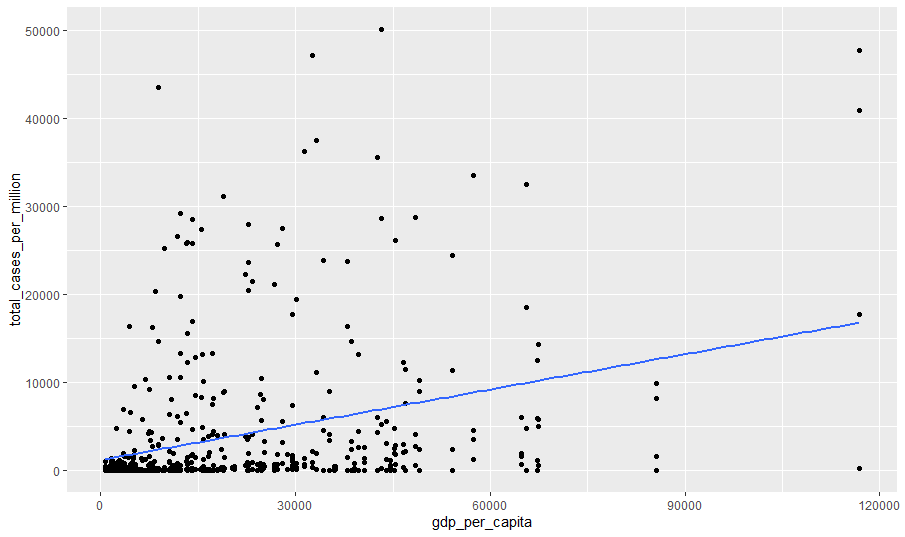
\includegraphics[width=\linewidth]{rys/mod10-lin.png}
	\caption{Wykres przedstawiający dopasowanie modelu liniowego}
	\label{fig:mod10-lin}
	\zrodlo{Opracowanie własne}
\end{figure}

Efekt PKB na osobę jest istotny statystycznie. Im wyższe PKB danego kraju, tym wyższa liczba zachorowań. 

\begin{table}[!htbp]
	\begin{center}
		\begin{tabular}{l c}
			\hline
			& Model 1 \\
			\hline
			(Intercept)          & $0.42$       \\
			& $(0.55)$     \\
			gdp\_per\_capita\^~0.2 & $0.79^{***}$ \\
			& $(0.08)$     \\
			\hline
			R$^2$                & $0.15$       \\
			Adj. R$^2$           & $0.15$       \\
			Num. obs.            & $531$        \\
			\hline
			\multicolumn{2}{l}{\scriptsize{$^{***}p<0.001$; $^{**}p<0.01$; $^{*}p<0.05$}}
		\end{tabular}
		\caption{Wyniki dla modelu 10 z przekształceniem zmiennych}
		\label{table:mod10-log}
	\end{center}
\end{table}

\begin{figure}[htbp]
	\centering
	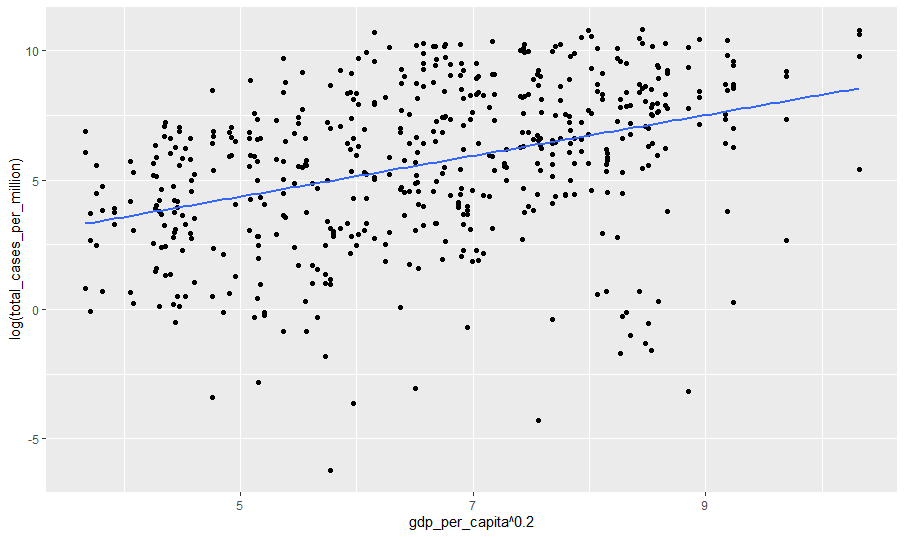
\includegraphics[width=\linewidth]{rys/mod10-log.png}
	\caption{Wykres przedstawiający dopasowanie modelu liniowego z przekształceniem zmiennych}
	\label{fig:mod10-log}
	\zrodlo{Opracowanie własne}
\end{figure}

\chapter*{Podsumowanie i~wnioski}

W tabeli \ref{tab:istotnosc} znajduje się podsumowanie istotności poszczególnych czynników, których wpływ na liczbę zachorowań był badany w tej pracy.


\begin{longtable}{| p{.30\textwidth} | p{.60\textwidth} |}
	\hline
	Cecha & Wpływ na liczbę zachorowań \\ \hline 
	Czas & istotny, wraz z upływem czasu rośnie liczba zachorowań \\ \hline
	Liczba wykonywanych testów na COVID-19 & istotny, wraz ze wzrostem liczby testów rośnie liczba zachorowań \\ \hline
	Oczekiwana długość życia & istotny, o ile ta wartość przekracza 80 lat, wówczas zachorowań jest więcej niż dla krajów o krótszej oczekiwanej długości życia \\ \hline 
	Gęstość zaludnienia & nieistotny \\ \hline
	Wskaźnik siły obostrzeń & istotny, im wyższy, tym mniej zachorowań \\ \hline
	Wskaźnik rozwoju społecznego & istotny, w krajach o wysokim wskaźniku rozwoju jest więcej zachorowań \\ \hline
	Śmiertelność z powodu chorób sercowych & istotny, im wyższy jest ten współczynnik, tym mniej zachorowań na COVID-19 \\ \hline
	Powszechność występowania cukrzycy & istotny, im wyższy jest ten współczynnik, tym więcej zachorowań na COVID-19 \\ \hline
	Część populacji żyjąca w skrajnym ubóstwie & istotny, im większa jest część mieszkańców żyjąca w biedzie, tym mniej zachorowań \\ \hline
	PKB na osobę & istotny, im wyższe PKB, tym więcej zachorowań \\ \hline
	\caption{Porównanie istotności i wpływu różnych czynników na liczbę zachorowań w przeciętnym kraju}
	
	\label{tab:istotnosc}
	
	\end{longtable}
\begin{center}\zrodlo{Opracowanie własne}
	\end{center}
\newpage

\begin{table}
	\centering
	\begin{tabular}{|c|c|}
		\hline 
		Nr modelu&   AIC \\ \hline
		1.1 &  715285\\ \hline
		1.2&  655232 \\ \hline
		2 &  363631  \\ \hline
		3 &   729555  \\ \hline
		4 &   729672  \\ \hline
		5 &   687061  \\ \hline
		6 &   720399  \\ \hline
		7 &   729657  \\ \hline
		8 &   729646 \\ \hline
		9 &   520055 \\ \hline
		10&   720911 \\ \hline
	\end{tabular}
\caption{Porównanie indeksów Akaike dla poszczególnych modeli}
\label{tab:akaike}
\zrodlo{Opracowanie własne}
\end{table}

Indeks Akaike jest miarą utraconej informacji. Im mniejszy jest indeks Akaike, tym lepiej model wyjaśnia badane zjawisko. Widzimy z tabeli \ref{tab:akaike}, że najmniejsze AIC występuje dla modelu nr 2. Jest to model, gdzie występuje zależność między liczbą zachorowań a liczbą wykonywanych testów. Ta zależność jest bardzo oczywista, ponieważ liczbę zachorowań zlicza się na podstawie tego, ile testów dało wynik pozytywny. Modelem z drugim najniższym AIC jest model nr 9, gdzie badamy istotność wskaźnika części populacji żyjącej w skrajnym ubóstwie.



Wszystkie modele jednoznacznie pokazują, że efekt kraju jako czynnika zakłócającego jest bardzo istotny, w wielu przypadkach wyjaśnia ponad połowę wariancji resztowej modelu, więc zmienność liczby zachorowań pomiędzy różnymi krajami jest około dwukrotnie większa niż zmienność liczby zachorowań w pojedynczym kraju.

Na to, co jest nazywane w tej pracy ,,efektem kraju'', składa się tak naprawdę wiele innych czynników, m. in. gęstość zaludnienia, sytuacja ekonomiczna danego kraju, odsetek osób z chorobami towarzyszącymi, rozkład wieku, jak również przyjęta strategia walki z koronawirusem, na którą z kolei składają się m. in. liczba wykonywanych testów, przepisy w sprawie zamykania szkół, miejsc publicznych, ograniczenie kontaktów międzyludzkich, i wiele innych.



\begin{thebibliography}{99}

\bibitem{biecek} Przemysław Biecek, \emph{Analiza danych z programem R. Modele liniowe z efektami stałymi, losowymi i mieszanymi}, Wydawnictwo Naukowe PWN, Wydanie II, Warszawa 2013
\bibitem{faraway} Julian J. Faraway, \emph{Extending the Linear Model with R. Generalized Linear, Mixed Effects and Nonparametric Regression Models. Second Edition}, CRC Press Taylor \& Francis  Group, 2016

\bibitem{owid} \url{https://ourworldindata.org/coronavirus}

\bibitem{stringency} \url{https://www.bsg.ox.ac.uk/research/research-projects/coronavirus-government-response-tracker} (dostęp 31.10.2020)

\bibitem{dollars} \url{https://ourworldindata.org/what-are-ppps} (dostęp 31.10.2020)

\bibitem{prediction} Welham, Sue \& Cullis, Brian \& Gogel, Beverley \& Gilmour, A.R. \& Thompson, Robin. \emph{Prediction in linear mixed models.} Australian \& New Zealand Journal of Statistics. vol. 46.  (2004). p.  325 - 347. 10.1111/j.1467-842X.2004.00334.x. 

\bibitem{experimental} Howard J. Seltman, \emph{Experimental Design and Analysis}, \url{http://www.stat.cmu.edu/~hseltman/309/Book/}

\bibitem{brief} \url{https://peerj.com/articles/4794/} (dostęp: 11.11.2020)

\end{thebibliography}



\listoffigures

\listoftables


\chapter*{Załączniki}
\begin{enumerate}
%\item Oświadczenie o oryginalności pracy i możliwości jej wykorzystania. 
%\item Opinia promotora na temat oryginalności pracy oraz w~sprawie dopuszczenia do obrony pracy dyplomowej.
%\item Potwierdzenie analizy antyplagiatowej.
\item Płyta CD z niniejszą pracą w wersji elektronicznej.
\end{enumerate}




\chapter*{Streszczenie (Summary)}

\bigskip
\bigskip

\begin{center}
  \textbf{\tytul}
\end{center}

W tej pracy przedstawione są pojęcia związane z modelami liniowymi z efektami stałymi i losowymi. Następnie opisane są badania własne na zbiorze danych dotyczącym rozprzestrzeniania się choroby COVID-19 w różnych krajach na świecie.


\bigskip

\begin{center}
  \textbf{\textit{\tytulangielski}}
\end{center}



\selecthyphenation{english}
{\it
In this paper, concepts related to linear models with fixed and random effects are presented. Then, our own research is described on the dataset on the spread of COVID-19 in various countries around the world.
}

\end{document}

